\documentclass[12pt,a4paper]{article}
\usepackage{thesiscommands}

%\drafttrue % or
\draftfalse

\author{Richard Littauer}

% to be executed with: lualatex --shell-escape -synctex=1 -interaction=nonstopmode "complete_thesis_new_2".tex
% last changed on 26.8.16 9h30

\begin{document}

\begin{titlepage}
	\begin{center}

		% Upper part of the page. The '~' is needed because \\
		% only works if a paragraph has started.
		
\includegraphics[width=0.25\textwidth]{eule.png}~\\[1cm]

		\textsc{\LARGE Saarland  University}\\[0.4cm]
		\textsc{\Large Department of Computational Linguistics}\\[1.5cm]

		\textsc{\LARGE Master's thesis Proposal}\vspace{0.5cm}

		% Title
		\HRule \\[0.55cm]

		{ \huge \bfseries Open Source Code

			 and\vspace{0.2cm}

			 Low Resource Languages}\vspace{0.5cm}

		\HRule \\[1.5cm]

		% Author and supervisor
		\begin{minipage}{0.45\textwidth}
			\begin{flushleft} \large
				\emph{Author:}\\
				Richard \textsc{Littauer}\\
				Matriculation: 2539658
			\end{flushleft}
		\end{minipage}
		\begin{minipage}{0.45\textwidth}
			\begin{flushright} \large
				\emph{Supervisors:} \\
				Dr. Dietrich \textsc{Klakow}\\
				Dr. Alexis \textsc{Palmer}\\
				% \emph{Advisors:} \\
				% Dr. Harm \textsc{Brouwer}\\
			\end{flushright}
		\end{minipage}

		\vfill

		% Bottom of the page
		{\large \today}

	\end{center}
\end{titlepage}
\newpage

\thispagestyle{empty}
\begin{abstract}
  \setlength{\parskip}{2ex plus 0.5ex minus 0.2ex}

  % Please put \noindent before each paragraph of the abstract!

  \noindent Of the roughly seven thousand languages currently spoken, less than fifty have a significant digital presence. In order for a language to be used digitally and to survive in the long term, it's speakers may need to develop computational resources: orthographies, dictionaries, grammars, spell checkers, parsers, and more. Instead of depending on closed source code from large providers, researchers and communities can leverage open source code as a means of bootstrapping digital language development. In this thesis, I discuss the state of the field for low-resource languages, what open source code is and how this methodology can help languages. I provide two cases studies, looking in detail at Gaelic and Naskapi, and I describe a database I have developed for open source code serving these languages. Looking to the future, I suggest steps for helping save languages from being lost.

  \noindent My specific contributions in this thesis include not only the first published analysis of open source code specifically regarding endangered languages, and an exposition of the only database of open source resources, but also the first independent fieldwork with Naskapi that pertains to its digital presence. I also outline how researchers and developers can change their processes to help make their work more effectual in the long term.

\end{abstract}


\newpage

%%% Eidesstattliche Erklärung
\thispagestyle{empty}
\noindent\textbf{Eidesstattliche Erkl\"arung}

\noindent Hiermit erkl\"are ich, dass ich die vorliegende Arbeit selbstständig verfasst und keine anderen als die angegebenen Quellen und Hilfsmittel verwendet habe.\\

\noindent\textbf{Declaration}

\noindent I hereby confirm that the thesis presented here is my own work, with all assistance acknowledged. \\

\noindent\textbf{Acknowledgements}

\noindent Jonathan Poitz provided formatting files, but did not advise on the content. This thesis is based loosely on a paper presented at the LREC CCURL Workshop in July 2016 in Slovenia \citep{CCURL}. Hugh Paterson III was a coauthor on that paper.

\vspace{1cm}

\noindent Montr\'eal, \thedate

\vspace{1.7cm}

\noindent Richard Littauer

%%% Eidesstattliche Erklärung End

\newpage
%
\tableofcontents
\thispagestyle{empty}
\addtocontents{toc}{\protect\thispagestyle{empty}}

\newpage

% % \listoffigures
% % \listoftables
% % \listoflistings
% % \thispagestyle{empty}
% % \newpage

\setcounter{page}{1}

% !TEX root = thesis.tex
\section{Introduction}
\label{sec:intro}

At least half of the world's 6000-odd languages will be extinct this century \citep{krauss92, grenoble_2011}. Just over half of these languages have writing systems.\footnote{\href{https://www.ethnologue.com/enterprise-faq/how-many-languages-world-are-unwritten-0}{https://www.ethnologue.com/enterprise-faq/how-many-languages-world-are-unwritten-0}} It is estimated that less than 5\% of the world's languages are used online or have significant digital presence \citep{kornai2013digital}. 

The majority of the world's computational technology has been built by English, with English manuals, English interfaces, and by English speakers. The most prevalent language spoken by users of this technology is also English. There are a few languages - around thirty - with the combination of large populations with internet access, official governmental status, and industrial economies which affords them some native computational technology, in particular on the World Wide Web, the largest global network for sharing code and written material.

English is the undisputed heavyweight as far as global written resources are concerned.\footnote{\href{https://w3techs.com/technologies/history\_overview/content\_language}{https://w3techs.com/technologies/history\_overview/content\_language}} Over half of the web's content is written in English. The next largest languages are Russian, German, Spanish, Japanese, and French - with a combined population of well over a billion speakers. Portuguese, Italian, and Chinese have the next largest amount of content - but each of them only covers between 2 and 3\% of the web's content - followed by Polish, Turkish, Dutch, and Korean with over 1\%. Suffice to say, the graph of global written content is not skewed towards language diversity as a norm. This is not surprising in any event, as around 90\% of the world's languages are spoken by less than 10\% of its people \citep{bernard1992preserving}.

In part, these high resource languages depend upon shared code. Put simply (and therefore ungracefully), a literacy system affords written corpora, and written corpora can be used by researchers to either build tools for that language or to adapt tools from other languages. These tools might be spell-checkers, parsers, input systems, or later on speech recognition and generation software, semantic analysers, or machine learning and translation systems, among others.

This culturally shared body of code is most often developed in closed environments with consumer endpoints, by the military or large businesses. For instance, the World Wide Web (from here on, the web), the largest shared corpus of written language, started with support from  the Massachusetts Institute of Technology (MIT) and the Defense Advanced Research Projects Agency (DARPA). (This helps to explain why most of the web is written in English.) Another example would be Google Translate, which uses massive bilingual corpora to provide automatic translation services for free online, but whose code is proprietary and owned by Google.

While the enterprise pathway works well for large languages where populations of speakers can be leveraged to provide funding, the majority of the world's languages are not able to develop their own computational resources - either grammars, corpora, or code. Instead, they must rely on small groups of researchers, limited funding, and a grab-bag of written resources when they have them. For instance, the most consistent translations cross-linguistically are of the Christian Bible, which may not reflect the target language's culture.

In this thesis, I will examine methodology that can be used by linguists, researchers, and language developers to help their languages "digitally ascend" (as \citet{kornai2013digital} puts it) - to bootstrap their corpora creation, write grammars, transform other language's tools and research to their own languages, and to ultimately enable their communities to speak and share their knowledge computationally. This methodology goes under the broad label of \textit{open source} software. Open source software is code which has been developed and made available for free, without concessions about how it is to be used or who uses it. This allows coders to use code which they personally haven't built without allocating funds for it, thus freeing up significant portions of research and development costs for making tools. At present, the majority of the world's code depends on some level on open source software - for instance, Linux, and much of the web, depends on open source code.

In the field of computational linguistics, however, there are a deficit of resources which are licensed and available as open source. This largely stems from the need to financially recoup expenses for development, on licenses mandated by research groups or military funders, and on a lack of awareness of how open source code works by developers. Another consideration is that an open source label does not ensure that the code is worth using, maintained, relevant, or in scope for a given domain.

Below, I will go into further depth about the state of endangered languages and computational resources in Section~\ref{sec:endlang}, and what different languages need in order to have digital presence in Section~\ref{sec:resources}. In Section~\ref{sec:open-source}, I'll define what open source is, and talk about issues relevant to open source code for under-resourced languages. I'll then in Section~\ref{sec:endlangcode} talk about the state of the open source ecosystem for low resource languages online, in particular focusing on a database of open source code that I have built with the help of researchers around the world.

I'll touch on some specific examples of languages which could benefit from open source code in Section~\ref{sec:case-studies}, focusing on Gaelic, an endangered language with tens of thousands of speakers but little online resources, and Naskapi, an endangered languages with only a thousand speakers which might be able to benefit from open source code. The Naskapi case study will be informed by original research, as I engaged in field research at the town where most Naskapi live and talked to linguists working on literacy efforts for this language. In Section~\ref{sec:methods}, I'll discuss how open source can help low resource languages, and in Section~\ref{sec:discussion} I'll expound further at a high level on what open source enables for linguists and language communities. Finally, in Section~\ref{sec:future-work} and Section~\ref{sec:conclusion} I'll discuss future work, and offer some concluding remarks.

% TODO Final draft: include accomplishments this thesis adds.

% !TEX root = thesis.tex
\section{Low Resource Languages: An Overview}\label{sec:endlang}

In this section, I will outline the state of low resource languages. First I will define contrasting and distinct terms which are often used to these languages, which inform how one can approach a language. Then, I will talk about language demographics and metrics used to categorise languages as having low resources, before moving on to discuss digital presence as a term for understanding language endangerment today. Finally, I'll go into depth further about the current state of language diversity (both in research and demographically), and mention the various different groups who work on and fund low resource development, and how considering their impact influences a language's digital presence.

\subsection{Definitions}

Before going further, it makes sense to define what the terms \emph{endangered}, \emph{minority}, \emph{low} and \emph{under-resourced}, and other terms like \emph{threatened} mean when they refer to a language. Ultimately, they refer as a whole to languages which are in peril in some way. However, there have slightly different meanings in different contexts, and according to the scale and metric applied.

In this section, I will generally define these terms: \textit{endangered}, \textit{moribund}, \textit{extinct}, \textit{dormant}, \textit{revitalised}, \textit{historic} and \textit{constructed} languages; \textit{minority}, \textit{low-resource}, \textit{under-resourced}, \textit{incident} and \textit{surprise} languages; and finally \textit{computer} or \textit{computational} languages. This will help inform why I've chosen to focus on low resource languages, and specifically low resource natural languages with living populations.

All of these terms are controversial, and work within larger frameworks and ontologies. I'll cover this in Subsection~\ref{subsec:metrics} on metrics after giving this general overview of definitions.

\subsubsection{Endangered, revitalised, and extinct languages}

\emph{Endangered} languages are human languages that are in danger of extinction. The term is borrowed from the scientific literature describing animals; just as there exists as very real possibility that one day there will be no more Australasian Bittern specimens in the wilds of Australia, it is also possible that one day there may be no living speakers of Guugu Yimithirr. The term is not complete analogous; we can still read Tocharian texts, but Tocharian is not considered to be a living language, but \textit{extinct}, as there are no speakers who use it regularly (and who are not scholars of obscure languages).

Endangered languages are normally languages which have a high amount of speakers, and crucially are still teaching children the language. Children ensure that the language will live on to the next generation, and when this chain breaks, it is almost impossible to resurrect a language. A language would be endangered when it can be assumed that children will stop learning the language in the next hundred years (according to \citet{krauss92}). This can be difficult to judge, as the rate of deterioration can be high. For instance, Breton had over a million speakers in 1950, but today the numbers may be as low as 200,000. Its future is uncertain.

\emph{Moribund} languages are languages which are critically endangered, in that there are no children currently learning the language and using it frequently, although there are speakers. Ainu is a good example, with roughly ten native speakers still living, all of whom are over 80 years old, \footnote{\href{https://www.ethnologue.com/language/ain}{https://www.ethnologue.com/language/ain}} although there are some struggling efforts to revive it \citep{hanks2017policy}. On the other side of the northern Pacific, Haida has a similar amount of native speakers, but because of the amount of immersion programmes, government-funded schools, and new venues for the language such as a motion picture filmed entirely in Haida with ethnically Haida actors who learned their lines from the elders, \footnote{\href{https://www.nytimes.com/2017/06/11/world/americas/reviving-a-lost-language-of-canada-through-film.html}{https://www.nytimes.com/2017/06/11/world/americas/reviving-a-lost-language-of-canada-through-film.html}} it is not considered moribund.

\emph{Dormant} or \textit{sleeping} languages are a stage beyond moribund languages. They have no living fluent speakers. This does not mean that the language is extinct. An example would be Mutsun, an Ohlone or Costanoan language formerly spoken near San Juan Bautista, California, whose last known fluent speaker Ascensi\'on Sol\'orsano passed away in 1930. However, in the late 90s, the Mutsun people (recognised formally as the Amah Mutsun Tribal Band) began a revitalisation project using the extensive documentation left behind by linguists, anthropologists, and a Catholic mission priest, and now there are several conversational (albeit no fluent) speakers \citep{warner2007ethics}. Ethnologue defines dormant as a language which has no speakers, but there is still a community that attaches its ethnic identity to the language \citep{lewis2010assessing}.

Often, dormant languages only come to attention when they are considered a \textit{revitalised} language. As \citet{warner2007ethics} notes, "Daryl Baldwin did indeed teach himself his then-dormant ancestral language, Myaamia, and is now raising his children largely in the language \citep{hinton2001sleeping, leonard2004acquisition}." Before Baldwin's work, Myaamia would have been considered a dormant language. Another example would be Manx, which lost all of its native speakers (the last being Ned Maddrell, who died in 1974 \citep{wilson2008revitalization}), but retained a score of second language speakers until today, when there are now immersion programmes for children and over a thousand speakers of the language \citep{clague2009manx}. Between 1974 and a vague point somewhere in the past couple of decades where a child could consider Manx as their first language, the language was dormant; now, however, it is revitalised.

The most famous example of a revitalised language is Hebrew, with a speaking population of over eight million,\footnote{\href{https://www.ethnologue.com/language/heb}{https://www.ethnologue.com/language/heb}} which was formerly a literary language until revitalisation efforts began as a result of the creation of the Israeli state in the early 20th century, where it is now an official language and not in a state of endangerment. Hebrew is a good example of why the often synonymous terms such as 'endangered' and 'revitalised' should be considered as differentiable.

While on the subject of Hebrew, it is worth mentioning that the initial efforts to revitalise it were often maligned by both Jewish communities and linguists, for a variety of reasons. First, the Jewish faith had traditionally viewed Hebrew as a holy tongue, and many religiously conservative Jews objected to the sacrilegious use of it for day-to-day matters, preferring Aramaic or Yiddish. Many also objected on the grounds that its use was connected to Zionism (why is well beyond the scope of this thesis). But most pertinently, linguists objected because they viewed revitalisation as an impossibility. If the language was dead, than it would be impossible to accurately bring it back, as literary texts are not sufficient at adequately capturing all of the intricacies of a language and how it is used. Clearly, with millions of first language speakers, this is no longer a valid point; these critics can now claim that modern Hebrew is an imperfect descendant of historical Hebrew, which remains extinct, and they are likely right to do so. Revitalisation is not always an ethically or logistically clear process.

This is especially true for \textit{constructed} languages, which are \textit{a priori} languages invented by a linguist or a community without a historical speaking community or lineage. These may be created to be logically resistant to ambiguity (such as Loglan or Lobjan \citep{okrent2009land}), for a specific artistic purpose (such as Na'vi or Klingon, meant to be spoken by aliens in science fiction \citep{schreyer2015digital, schreyer2011media}), for scientific study (such as those used by evolutionary linguists for language games with participants to discern how language might have evolved \citep{scott2010language}, or such as used in the ubiquitous Wug test by scholars of language acquisition \citep{ratner2000beginning}) or for political aims (such as Esperanto or Ido \citep{okrent2009land}). Some of these may end up with thousands of speakers, including native speakers, and a huge surplus of computational resources. Na'vi has a dictionary that has been translated using computational tooling into over a dozen languages, for instance, and morphological parser, spell checkers, and a Facebook translator. These languages are not normally considered as revitalised or dormant, but are instead mostly ignored or actively excluded (see \citet{gibson2016assessing} for an example of this) by the scientific community altogether.

Heading back to natural languages, Latin would largely not be considered a revitalised language either, although there are immersion schools and some daily usage by the Catholic liturgy. These domains are specific and do not extend into normal life, on the whole. This doesn't mean it doesn't have some computational resources, however - the ATMs in the Vatican use Latin as a user interface language.\footnote{\href{https://gizmodo.com/5905595/the-atms-in-vatican-city-speak-latin}{https://gizmodo.com/5905595/the-atms-in-vatican-city-speak-latin}} Old Swedish, likewise, has some computational resources (admittedly, from a single research group that is humorously aware of the lack of general global interest in the field).\footnote{\href{https://spraakbanken.gu.se/swe/forskning/diabase}{https://spraakbanken.gu.se/swe/forskning/diabase}} Latin would normally be considered a \textit{historic} language, like Ancient Greek or Old English. All of these languages, while extinct themselves, have direct descendants (the Romance languages, modern Greek, and English, respectively), but this is not always the case.

Gothic is considered \textit{extinct} today, as it has no direct descendants, although it is still studied, and although there is a small community of writers who continue to use the language, and at least one publishing company which publishes modern work in Gothic\footnote{\href{https://wordhoardpress.com}{https://wordhoardpress.com}} (incidentally run by, of all people, me). Not all languages have sufficient texts to be revitalised or used today: Etruscan, Minoan, and Pictish are good examples.

One could argue that some languages may be considered dormant even if there are native speakers alive, if they do not speak the language. For instance, there are a few cases where a couple of speakers are left of a language, but they don't speak it to each other due to interpersonal differences. Most famously, there is the apocryphal story of Ayapeneco, where a global m\^eme ensued from an imagined feud between the last two speakers, to the point where Vodafone released a video claiming that they helped bring the men together to save the language (to the chagrin of actual linguists and anthropologists who had worked on the language for decades).\footnote{\href{http://stories.schwa-fire.com/who\_save\_ayapaneco\#chapter-113060}{http://stories.schwa-fire.com/who\_save\_ayapaneco\#chapter-113060}} This has actually happened elsewhere, such as with Nisenan \citep{snyder2004practice}. Another example might be Ishi, the last Yahi and a speaker of Yana, who explained that he had no name, because there was no other Yahi man to formally introduce him. Ishi means 'man' in Yana, and is what Ishi consented to be called as a placeholder for his actual name \citep{kroeber1973ishi}.

Such cases are extreme, and there will be exceptions to almost any of these categories. Even for living languages, questions of identification can be difficult. For instance, \cite{gilRiau} points to at least a dozen different interpretations of what Riau Indonesian might technically be. Defining language is beyond the scope of this thesis - however, I would be amiss not to mention this problem here.

\subsubsection{Official, \textit{de facto}, \textit{de jure}, majority, and minority languages}

All of the former definitions were seen through the lens of language communities and vitality. However, there are other lenses through which languages as a whole can be viewed - for instance, politically and computationally.

Political definitions of language include \textit{official} and \textit{working} languages. Official languages are languages which are given a definitive status by a state, normally on the national level. On the supranational level (such as is the case with the EU or the ICC), they are generally termed working languages (which is different, in turn, from a \textit{lingua franca}, which is a trade, bridge or link language used informally between groups who speak different languages themselves). These languages can be broken down into {\it de facto} an {\it de jure} languages - the latter are given legal status in the law, while the former do not have official legal status but are considered culturally and for most intents and purposes as the legal language. An example would be in the United States, where there is no {\it de jure} legal language, but the {\it de facto} language is English. This means that most resources are provided in English, and other languages are often ignored or not allocated resources by the law.

\begin{quote}
These terms, as defined by \citet{johnson2013language}, distinguish policies from one another by virtue of their alignment between law and practice, respectively. Here, {\it de jure} policies are those disseminated in legal proclamations, typically being 'officially documented in writing' (p. 10). By contrast, {\it de facto} policy describes those policies that exist in {\it practice} [sic], crucially, without legal provenance or even {\it in spite} of existing \textit{de jure} polices. \citep{hanks2017policy}
\end{quote}

An example given by \citet{hanks2017policy} is the case of boarding schools in the United States and Canada for indigenous children, often forcibly removed from their home, where the {\it de jure} goal was to provide the children with a working knowledge of English, but the {\it de facto} result was that they were heavily discouraged (often through direct physical abuse to students who spoke in their language) from speaking their native tongues in the classroom or in the schools, with the result that many languages were directly endangered or lost. This has happened in many places, as well: for instance, Gaelic was forbidden in the classroom by English teachers, and children were beaten (for instance, slapped across the knuckles with a ruler) for using Gaelic.

Within a state, the proportion of population of speakers compared to the entire population generally determines wether a language is considered a \textit{majority} or a \textit{minority} language. Not all minority languages are endangered languages; for instance, Catalan, spoken by around nine million people in Catalonia and southern France, is not endangered, although it is a minority language and is not an official language of any country. There are arguments that it is the majority language for a stateless state. The same could be said of Tibetan, which is officially the minority language in a region of China, but is considered the be the majority language of the region of Tibet itself, which many view as its own state currently under illegal occupation (as with Hebrew and Israel, further political discussion is beyond the scope of this thesis.)

Some minority languages have legal status as minority languages. A good example would be in Canada, where minority languages in each province are given legal protection - for instance, English in Qu\'ebec, where a majority of the speakers are Francophone, or French in Ontario, where the majority of the speakers are French. Sometimes languages with very small populations - such as indigenous languages spoken by First Nations communities in Canada - are given legal status, too, as is the case with Nunavut, a territory in Canada where two Inuit languages - Inuktitut and Inuinnaqtun - are granted legal status, although they are nationally minority languages, and although one of them, Inuinnaqtun, has less than 300 speakers and comprises only around 1\% of the population of Nunavut. Another example would be Hawai'ian, which is the state language of Hawai'i since 1978, although it only has around 2000 native speakers, and is a minority language in Hawai'i.


\subsubsection{Low resource, under resourced and incident languages}

\textit{Low resource} languages are languages which have fewer computational resources than any of the bigger languages that dominate global discourse. There is no distinct cut-off for defining a low resource language versus a \textit{high resource}, \textit{resource-rich}, or just a \textit{resourced} language. A \textit{low resource} language can also be indiscriminately called a \textit{under resourced}, \textit{sparsely resourced}, or \textit{sparse} language. The disparity in resolved definitions reflects the focus of research, as generally researchers work with specific languages on computational models, and not on large databases where a precise definition is useful. Qualifiers are often included - for instance, \citet{agic2015if}'s paper, "If all you have is a bit of the Bible: Learning POS taggers for truly low-resource languages." These qualifiers are generally not considered within a rigorous system of rank - for more on that, consider Section~\ref{subsec:metrics} on metrics below.

In the context of low resource languages, the majority of established work revolves around adapting existing systems from high resourced languages to low resource languages. In such a case, the \textit{source} language is where the original system was originally trained or upon which it was built, while the \textit{target} language is the language upon which the system is being used, tested, or adapted. These terms are largely context dependent. Similarly, \textit{sparse} in particular is more often used to refer to a dataset, but can be used of a language when it is under resourced.

While hypothetically some languages could be defined as having no resources, there is no commonly used term such as 'resourceless'. In general, languages without writing systems fit in this category, and while it would potentially be interesting to train resources on audio-only vocabulary, this is generally not done computationally, but intensively by field linguists using specific tools such as dictionary applications or audio/video applications such as Praat \citep{boersma2009praat}, which allows you to view the waveforms for spoken corpora and annotate it. These resources - annotated (or not) corpora made by field linguists for a language - are, along with word lists and basic dictionaries, often the first resources for a given language, and are often not published but are accessibly only through corresponding with the linguist or team doing the work. A comparison with multimillion dollar projects such as Google Translate makes it clear that these languages would be considered under resourced.

Another couple of terms often used in this general context are \textit{incident} or \textit{surprise} languages. The latter is generally used for challenges, and was first used to describe the US Defense Advanced Research Projects Agency (DARPA) "Surprise Language Challenge", run by their Translingual Information Detection Extraction and Summarization (TIDES) programme in 2003. The challengee's goal was to see if a teams working on new languages they hadn't seen before (hence, 'surprise') could develop sufficiently useful resources and machine translation systems within a constrained period of time. \citep{oard2003surprise} These sorts of challenges aren't limited to DARPA; for instance, there was a Workshop on statistical Machine Translation held at EMNLP 2011 \citep{callison2011findings}. This workshop focused on a few tasks, one of which was based on the successful efforts by the Microsoft Translation team in 2010 to build a machine translation system for Haitian Creole that used SMS messages, after an earthquake there precipitated the need for a translation system between aid workers and spekaers of Haitian Creole, previously a low resource language \citep{lewis2010haitian, lewis2011crisis}. Haitian Creole, here, would be an \textit{incident} language.

\subsubsection{Computer languages}

A \textit{computer} or \textit{computational} language is a formalised language used to communicate instructions to a machine. There are a large variety of names and variants, and the definition here may be construed as insufficient. For the purposes of this thesis, a computer language is for talking to a machine, and is demonstrably different than a human language, which is generally used for communicating with humans. This definition is important only in so much as it helps clarify that we are talking about human languages when we mean low resource or endangered languages, not computer languages. The relevancy, usage, or status of computer languages is largely irrelevant here, unless it touches on resources used on human languages. For instance, any grammar written in COBOL, a sixty year old language, may be less accessible to open source coders who write primarily in Python or JavaScript, two popular languages used on the web and in the FLOSS ecosystem today. This type of situation will be covered in more depth in Section~\ref{subsec:digital-permanence}.

Other terms used in exploring the theory of language, semiotics, or formal language theory - such as context-free or recursively-enumerable languages - are outside of the scope of this thesis unless they touch on human and low resource languages directly in some tangible way.

\subsection{Metrics for language vitality}
\label{subsec:metrics}

Language health or vitality is a topic of increasing scholarship and interest. Superficially, it makes sense to use a similar system to classify languages as one would classify biological species, using the metrics defined by the International Union for Conservation of Nature (IUCN)\footnote{\href{http://www.iucnredlist.org/}{http://www.iucnredlist.org/}}. They have nine levels of classification: Extinct, Extinct in the Wild, Critically Endangered, Endangered, Vulnerable, Near Threatened, Least Concern, Data Deficient and Not Evaluated. However, the system is not directly transferable - how would a dormant language be classified? One can see immediately that there is a need for a language-specific rating system.

It is perhaps unsurprising that there are various metrics which can be used to classify the health of a language and its community. In this section, I'll explain these metrics in detail, focusing on the GIDS, EGIDS, UNESCO, and LEI measurements, as suggested by \citet{yang2017toward} as the main players in the field.

\subsubsection{The Graded Intergenerational Disruption Scale (GIDS)}

The Graded Intergenerational Disruption Scale, developed by \citet{fishman1991reversing}, is the earliest and most well known of the scales. It rates languages based on their domains of use, and on the amount of passing on and education which continues to the next generation through the parents. Figure~\ref{fig:gids} summarizes the different stages. Generally, as a language progresses and becomes more imperilled, it ends up further down the list. As a language ceases to be used in one domain, it becomes less likely that it will in the future, and more likely that parents will consider the language to be less useful than another. Over time, this causes the language to lose speakers (although the process is not inevitable; for examples, language policy in Quebec helped secure and revitalise the language over the past half century \citep{bourhis2001reversing}).

\begin{figure}
 \centering
 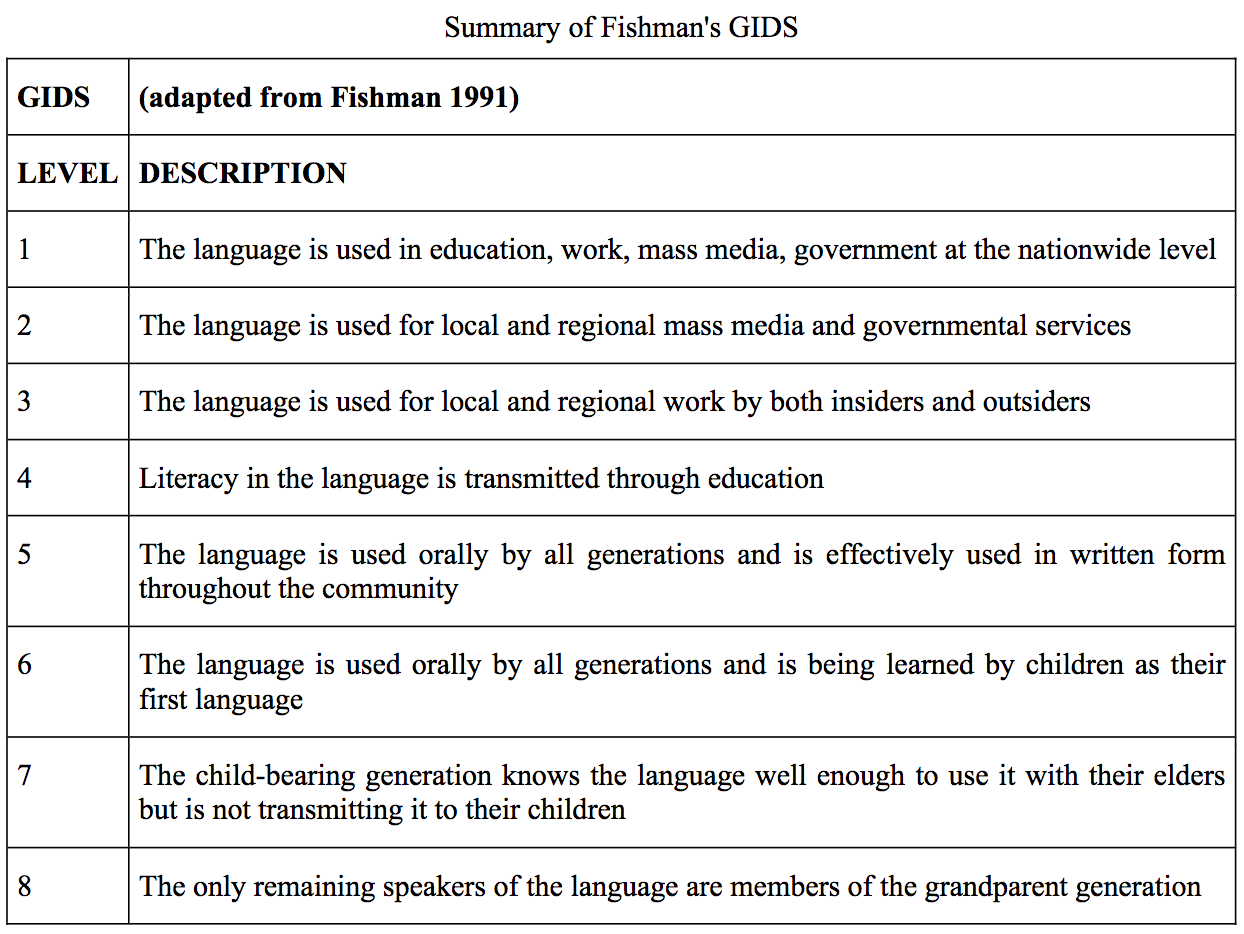
\includegraphics[width=.8\textwidth]{img/gids.png}
 \caption{A summary of GIDS from \citep{lewis2010assessing}}
 \label{fig:gids}
\end{figure}

\subsubsection{The UNESCO measurement scale}
\label{subsec:unesco}

Chronologically, the UNESCO rating was the next major scale in the field. The United Nations Educational, Scientific and Cultural Organization (UNESCO) is a specialised agency of the United Nations. In 2001, at the 31st Session of the UNESCO General Conference, they officially recognised that biodiversity, cultural diversity, and linguistic diversity are related. This viewpoint is relatively recent, and reflects increasing appreciation that culturally diverse regions tend to collocate with biodiverse regions, and that saving diversity implies saving both \citep{nettle2000vanishing, maffi2001biocultural, anderson2006language, krauss2007keynote, gorenflo2012co} (as discussed explicitly in \citet{maffi2001}, of which all of the authors were also members of the UNESCO Ad Hoc Expert Group on Endangered Languages). Encouragingly, UNESCO clarified at this event that sustaining and encouraging linguistic diversity lies within their charter.

In their publication from that conference, \citet{brenzinger2003language} lay out nine different metrics for measuring language vitality: six evaluate the vitality and state of endangerment, two language attitudes, and one related to urgency of documentation. The UNESCO system is rigorous in its refusal to apply a single score to a language, as that would smooth over the complexities of language usage. The six factors for vitality are: intergenerational language transmission (as with GIDS), absolute number of speakers, proportion of speakers within the total population, trends in existing language domains, response to new domains and media, and materials for language education and literacy.

For each of these, they further break rating down into categories. For instance, when regarding intergenerational language transmission, they specify six different possible ratings - safe, unsafe, definitively endangered, severely endangered, critically endangered, and extinct - and equate each rating with a score from 5 to 0. Here one of the primary issues with the UNESCO rating can be seen  (as pointed out by \citet{lewis2010assessing}) - namely, that 'safe' is an incredibly large category that needs more fine-grained categories, as it would account for any GIDS-rated language above Level 6.

The three other factors they consider are: governmental and institutional language attitudes and policies including official status and use; community members' attitudes toward their own language; and the amount and quality of documentation. Each of these is also rated on a null to five scale. For documentation, only a superlative rating of five would be considered to be more than low-resourced, as a four rating would be given to a language where "There are one good grammar and a number of adequate grammars, dictionaries, texts, literature, and occasionally updated everyday media; adequate annotated high-quality audio and video recordings." Although useful for linguists wishing to work in the language, this may not be enough for useful analysis and use by computational linguists. %TODO Should there be a section about linguists vs computational resources?

In Figure~\ref{fig:unesco}, an example rating using this system, from the appendix of \citet{brenzinger2003language} itself, is included to get some grasp of how these grades work in parallel.

Importantly, UNESCO clarifies that it does not suggest using one metric over another, and that adding up the numbers in the scales - however easy that might seem, as all of the measurements except speaking population are scalar and hold the same number of levels - would be insufficient and not ideal. "\textbf{Languages cannot be assessed simply by adding the numbers
}; we therefore suggest such simple addition \textit{not be done} [sic]."

\begin{figure}
 \centering
 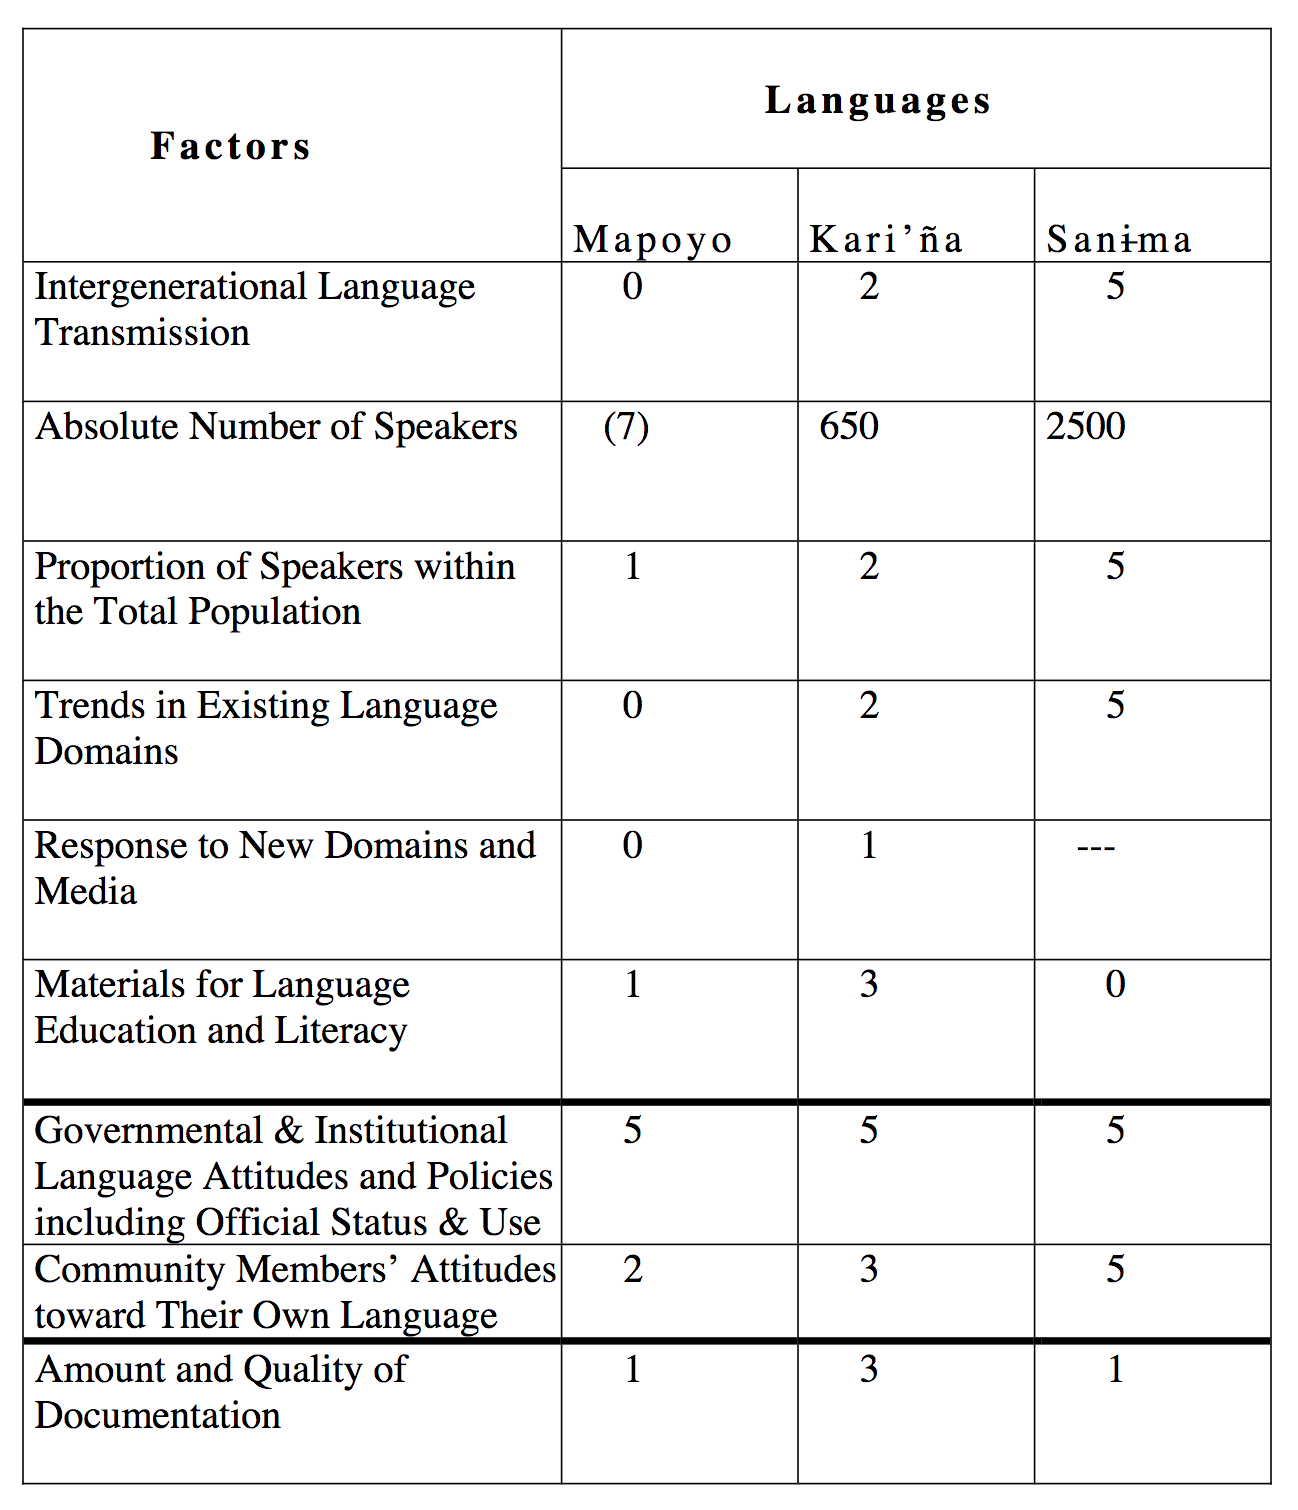
\includegraphics[width=.5\textwidth]{img/unesco.png}
 \caption{The UNESCO grading for three languages \citep{brenzinger2003language}}
 \label{fig:unesco}
\end{figure}

The UNESCO ratings for languages are listed in the \textit{UNESCO Atlas of the World's Languages in Danger} \citep{unesco2014unesco}.

\subsubsection{The Extended GIDS (EGIDS)}

Lewis and Simons, the authors of Ethnologue \citep{lewis2009ethnologue}\footnote{Also a website available at \href{https://www.ethnologue.com/}{https://www.ethnologue.com/}.}, pointed out some of the issues with GIDS which necessitate the creation of a new standard, and which could also eclipse or inform the UNESCO rating \citep{lewis2010assessing}. First, the levels are static, and don't account for directionality on the part of a language community up or down the strata. Second, there are language types which aren't included - for instance, there isn't a supranational level for extremely well-off languages, nor is there are level for extinct or dormant languages. Thirdly, GIDS focuses on intergenerational disruption in Level 5 and down, but in Level 4 and higher it focuses more on institutions, and this isn't accounted for well enough in the framework, which primarily focuses on parents as being the primary agents of language transmissions. Finally, the lower levels are not granular enough to cover the many complexities needed for language revitalisation groups.

EGIDS - the Expanded GIDS - serves these needs by providing more granular definitions. It also draws on the extensive knowledge of languages and their usage provided not only by Ethnologue, but also by the UNESCO Atlas and the community of linguists working with the Summer Institute of Linguistics (SIL), who fund and published Ethnologue. Figure~\ref{table:egids} shows the main categories, taken from the Ethnologue website\footnote{\href{https://www.ethnologue.com/about/language-status}{https://www.ethnologue.com/about/language-status}}. The table has been updated since \citet{lewis2010assessing}, in particular to also account for signed languages \citep{bickford2015rating}. The addition of a Level 0 and two levels beneath the scale are evident, as well as more granularity in the GIDS scale, such as can be seen with Level 6, which now has two levels, Level 6a Vigorous and Level 6b Threatened.

\begin{table}
\begin{center}
\begin{tabular}{|p{1cm}|p{3cm}|p{10cm}|} \hline
\textbf{Level}	& \textbf{Label}	& \textbf{Description} \\ \hline
0 	& International &  	The language is widely used between nations in trade, knowledge exchange, and international policy. \\ \hline
1 	& National &  	The language is used in education, work, mass media, and government at the national level. \\ \hline
2 	& Provincial &  	The language is used in education, work, mass media, and government within major administrative subdivisions of a nation. \\ \hline
3 	& Wider &  Communication 	The language is used in work and mass media without official status to transcend language differences across a region. \\ \hline
4 	& Educational &  	The language is in vigorous use, with standardization and literature being sustained through a widespread system of institutionally supported education. \\ \hline
5 	& Developing &  	The language is in vigorous use, with literature in a standardized form being used by some though this is not yet widespread or sustainable. \\ \hline
6a 	& Vigorous &  	The language is used for face-to-face communication by all generations and the situation is sustainable. \\ \hline
6b 	& Threatened &  	The language is used for face-to-face communication within all generations, but it is losing users. \\ \hline
7 	& Shifting &  	The child-bearing generation can use the language among themselves, but it is not being transmitted to children. \\ \hline
8a 	& Moribund &  	The only remaining active users of the language are members of the grandparent generation and older. \\ \hline
8b 	& Nearly &  Extinct 	The only remaining users of the language are members of the grandparent generation or older who have little opportunity to use the language. \\ \hline
9 	& Dormant &  	The language serves as a reminder of heritage identity for an ethnic community, but no one has more than symbolic proficiency. \\ \hline
10 	& Extinct &  	The language is no longer used and no one retains a sense of ethnic identity associated with the language. \\ \hline
\end{tabular}
\end{center}
\caption{Expanded Graded Intergenerational Disruption Scale}
\label{table:egids}
\end{table}

\citet{lewis2010assessing} also add another set of EGID levels which can be used to rate a language which is ascending in domains due to revitalisation efforts, which Figure~\ref{fig:egids-up} shows. This is generally useful, although it does suggest that a language uniformly descends or ascends, which may not be the case. The authors also spend time describing how to identify a language and decide which level best describes it.

\begin{figure}
 \centering
 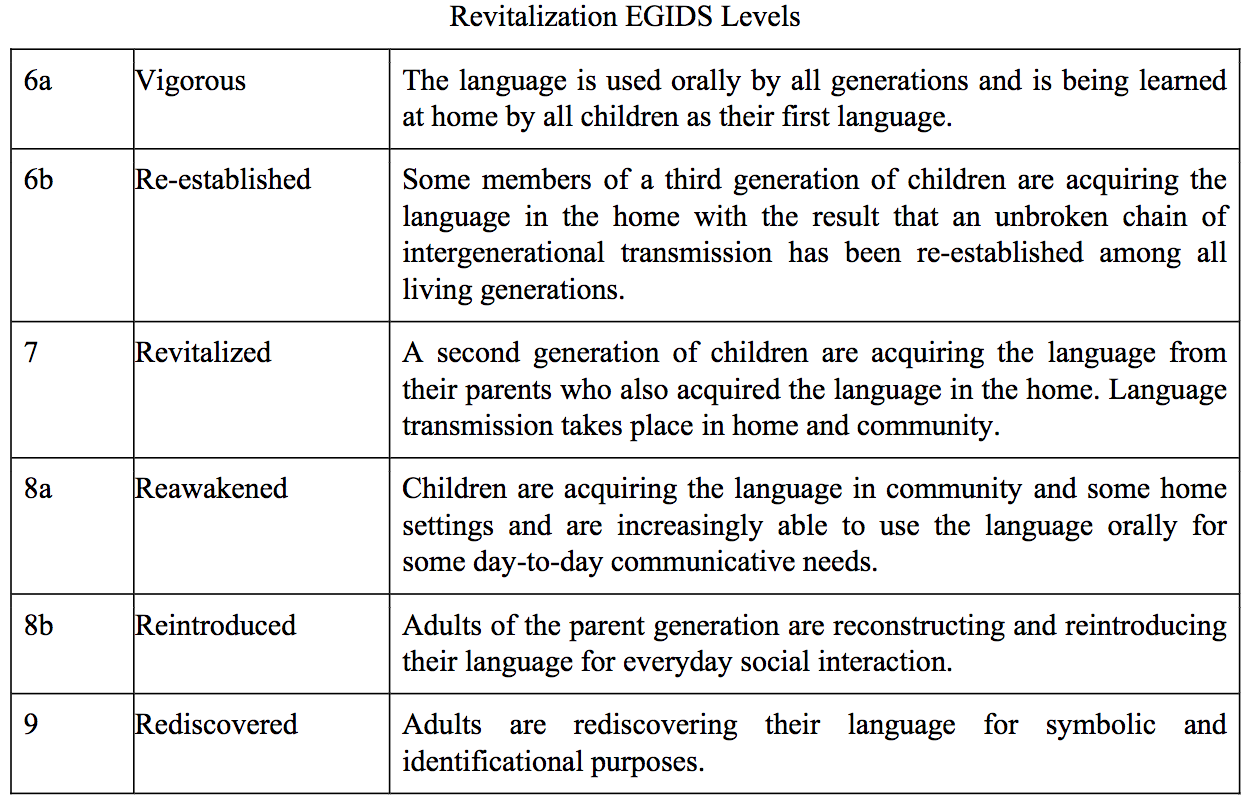
\includegraphics[width=.8\textwidth]{img/egids-up.png}
 \caption{A summary of EGIDS ascending levels from \citep{lewis2010assessing}}
 \label{fig:egids-up}
\end{figure}

They end with a quote from \citet{fishman2001can}, which explains further the purpose of EGIDS:

\begin{quote}
Thus, any theory and practice of assistance to threatened languages-whether the threat be a threat to their very lives, on the one hand, or a much less serious functional threat, on  the  other  hand-must  begin  with  a  model  of  the  functional  diversification  of languages. If analysts can appropriately identify the functions that are endangered as a result of the impact of stronger languages and cultures on weaker ones, then it may become easier to recommend which therapeutic steps must be undertaken in order to counteract any injurious impact that occurs. The purpose of our analyses must be to understand, limit and rectify the societal loss of functionality in the weaker language when  two  languages  interact  and  compete  for  the  same  functions within  the  same
ethnocultural  community  and  to  differentiate  between  life-threatening  and  non-life-threatening losses.
\end{quote}

\subsubsection{The Language Endangerment Index (LEI)}

Just as EGIDS expanded on GIDS, the Language Endangerment Index (LEI) was formed to resolve some of the issues with EGIDS, as well as to respond to GIDS, the UNESCO rating, and the rating in \citet{krauss2007classification} which focused almost exclusively on different ages of speakers and classified all languages with children speakers as 'stable', and all with over a million speakers as 'safe'. \citet{lee2016assessing} describe LEI for its use in The Catalogue of Endangered Languages (ELCat), part of the Google-powered Endangered Languages Project\footnote{\href{endangeredlanguages.com}{endangeredlanguages.com}}. The project isn't only sponsored by Google, but also by an American governmental National Science Foundation (NSF) grant\footnote{\href{https://www.nsf.gov/awardsearch/showAward?AWD\_ID=1058096}{https://www.nsf.gov/awardsearch/showAward?AWD\_ID=1058096}}, and is an ambitious project (like UNESCO and Ethnologue) to catalogue all languages and to provide specific metrics of language vitality.

The authors, in describing LEI, go into detail explaining how previous classifications, while they "highlight[s] the immensity of the problem at hand", can not easily apply to certain languages, and that these exceptions are critical to understanding whether the metrics are useful as opposed to being exceptions which prove the rule. Unlike the other papers, they explicitly mention some languages. For instance, they mention how \citet{dwyer2012tools} points out that Wutun, a Chinese-Tibetan-Mongolic language, is endangered due to a variety of factors, even if transgenerational transmission is not at risk - thus, GIDS or EGIDS may not satisfactorily categorise the language. A similar case could be made for Naskapi (see Section~\ref{sec:naskapi} for more on this).

The LEI uses four factors: intergenerational transmission, absolute number of speakers, speaker number trends (whether increasing or decreasing), and domains of use. Each of these is rated, like the UNESCO rating on a scale from null to five - however, unlike UNESCO, they add these numbers up to produce a single rating. The higher it is, the more likely the language is endangered. The scales are also somewhat different; for instance, number of speakers runs on orders of magnitude, with 100,000 being the top bound for a safe language (and not a million, like in \citet{krauss2007classification}).

\subsubsection{A response to qualitative metrics}
\label{subsubsec:response}

\citet{lee2016assessing} point out further issues with some of the other assessments - most notably that "while the UNESCO framework is broad and its factors comprehensive, it does not give an overall vitality score to the language being assessed, making it difficult to compare accurately across different language" and that "while an assessment of the type and quality of documentation is doubtlessly important because it helps indicate the potential for revitalization and the urgency of further research, it is not clear that the type and quality of documentation directly affects the vitality of a language." These two points are interesting, because they reflect how the situation of \citet{lee2016assessing} influences their judgement and their decision in making LEI at all. The authors were aware that they were being overtly quantitative in their approach:

\begin{quote}
Some may prefer a more nuanced examination of a language's vitality, with the view that the factors responsible for a language's endangerment are too complex to be compared across languages. Researchers of this view would rally against quantitative measures, stating that quantitative measures can hardly be accurate. ... ELCat researchers, while sympathetic to these points of view, maintain that without understanding and investigating fundamental common factors responsible for language endangerment, very little progress will be made in assessing language vitality and, consequently, less can be done to help communities preserve their languages. ELCat strikes a balance between these different perspectives.
\end{quote}

As \citet{grenoble2016response} points out, this misses the point of qualitative rebuttals, by claiming that accuracy is the most salient argument. It doesn't have to be, as there are more pressing concerns. For instance, and as \citet{grenoble2016response} points out, all of the metrics were built on the assumptions that quantifying language endangerment is useful, and that assessment directly leads to empowering communities to revitalise their language. Neither of these are directly backed up by empirical research. More pressingly, language itself is not indisputably something that is countable or measurable, and to think so is to reflect Western, modernist ideologies surrounding language, viewing a language as a distinct entity which is formalised in writing and education. Language could be viewed alternatively as inextricable from the speaker and the utterance, and this view is more likely to be taken by language groups which view themselves as separate from a nation-state or an ethnographic group \citep{bodo2017language}. To view language otherwise is to confine language to a countable, commodifiable entity in a post-colonial sense, which affects how the language is viewed and can have real effects on language communities. Even viewing linguistic biodiversity as something to be 'saved' raises ideological  concerns, as Haspelmath (one of the main editors of \citet{wals}) notes. \footnote{\href{dlc.hypotheses.org/195}{dlc.hypotheses.org/195}} Indeed, post-colonial attitudes towards language endangerment may be endemic; \citet{newman1998we} certainly suggests that non-Western linguists cannot adequately document or revitalise their own languages without Western training, which presupposes that to be an informed researched one must also conform to Western ideologies. Against this backdrop, \citet{lee2016assessing}'s claims that accuracy is something that can be attained seems to miss the mark; rather, the canonical approach to metrics is in itself a flawed approach that carries with it certain uncomfortable presumptions.

This thesis cannot hope to resolve these issues, nor is it meant to be an overview of the field of language vitality or endangerment as ideology. However, it is worth noting that metrics of language vitality do not exist in a vacuum, and that documentation and computational efforts are also a part of wider questions. Literacy is not a domain into which a language has to ascend to be seen as 'safe' or 'vital', and technological progress should not be viewed independently of an assessment of what exactly progress is.

Some things can be done, however. Terminologically, 'low-resource' is intentionally somewhat neutral, as compared to 'minority', 'endangered', or other terms that reflect Western viewpoints. Similarly, using the term language vitality as opposed to language endangerment "represents a significant shift in the representation of attitudes toward the rhetoric of indigenous languages to one away from dire predictions about endangerment to action-oriented attitudes about vitality and sustainability \citep{grenoble2016response}." These terms will be used for the rest of the paper, and any statements about resource development should be viewed as part of a narrower question of digital development (in the sense of building resources) for a specific, almost na\"ively countable view of language, unless otherwise specified (as in Section~\ref{sec:case-studies}).

% TODO Alexis: would be interesting to also discuss how these metrics might apply for the set of languages you're interested in (as defined in 2.1)

% Alexis: yes, in fact I think it's rather a different enterprise than defining language endangerment -- you may want to explicitly address the interaction between the two. what is your stance on the question? does lack of digital presence necessarily equate to language endangerment? (I think it's a very interesting question)


\subsection{Digital presence}

% I'll describe his assessment here, and explain why an alternative assessment would also be good. For instance, Wikipedia is, in my opinion, not a good judge of a language's health, as it is a closed ecosystem with diminishing returns for users who are bilingual.

Digital presence, briefly alluded to previously, can be thought of as the amount of language data available through digital sources. A looser definition could be 'the amount of written text on the web', but this would miss out on several important considerations. First, linguistic data does not have to be written to be digitally encoded; videos and audio data are both examples of digital content which is often digitally encoded. In some cases, pictures are also relevant, especially for signed languages or for examples of written text, such as in the millions of scans of papyrus from the Egyptian city of Oxyrhynchus, which are being translated using a crowd-sourced system by thousands of volunteers \citep{williams2014computational}, or for other language mediums, such as the khipu knot system used by the pre-Columbian Incan civilisation \citep{quilter2002narrative}. Secondly, the web (hereafter meant to refer to the World Wide Web) is not the only corpus of knowledge, nor is it the only network through which data can be accessed. Trivial example of other corpuses would be local files collected by individual field researchers that are backed up on hard drives; a similar example of another network would be a local area network in offline areas, or a university intranet.

However, the digital sphere can best be thought of schematically as a new domain for language use, and it is overwhelmingly today represented on the web. Ten years ago, it was fashionable to include references to the web "as a a corpus" (as \citet{scannell2007crubadan}, for instance, cited \citep{resnik1999mining, ghani2001mining, kilgarriff2001web}, although the latter two were in reference to low-resource languages); today, it is more common to cite studies on digital natives such as the 20,000 citation-strong \citet{prensky2001digital} paper\footnote{This number is from Google Scholar (\href{https://scholar.google.com}{https://scholar.google.com}) accessed April 9, 2018.}, or to assume that the web, and occasionally phone networks, are the main locations for digital communication. The web is ubiquitous; not only are more than half of the global population connected to the internet\footnote{\href{https://www.internetworldstats.com/stats.htm}{https://www.internetworldstats.com/stats.htm}}, but the internet, in developed countries, is used for all levels of communication, such as education, work, mass media, and in the home and local communities. Digital presence, then, is functionally the amount of usage on the web.

\subsubsection{Finding resources}
\label{subsec:finding-resources}

There are several resources which can be used to judge the amount of corpora for a language on the web, outside of papers defining metrics to judge these languages and to state whether they are endangered or thriving. The main resource for low resource languages is almost certainly the Cr\'ubad\'an project, developed by \citet{scannell2007crubadan}.\footnote{\href{http://crubadan.org/}{http://crubadan.org/}} This is a massive crawler which looks for documents with trigram frequencies for particular languages by checking against a seed corpus for under-resourced languages developed from Wikipedia, the Jehovah's Witness translations, and translations of the UN Declaration of Human Rights (UNHR). It is (to this author's knowledge) often the only corpus for a low resource language on the web, as is the case with Naskapi (see Section~\ref{sec:naskapi}).

Often, a translated Bible is the next best place to look for digital content. Biblical translations are so common as a first resource that there is a body of research that uses partial or full translations of the Bible for training NLP systems as a result \citep{chew2006evaluation}. However, finding the bible or UNHR is often difficult. In these cases, it is best to look for aggregators of data. There are a non-trivial number of large organisations and databases where it is possible to find resources - dictionaries, references, and occasionally software - on low resource languages.

\begin{itemize}

\item The Endangered Languages Project (ELP), described above and in \citet{lee2016assessing} and online\footnote{\href{http://www.endangeredlanguages.com/}{http://www.endangeredlanguages.com/}} has information on many under resourced languages.

\item Ethnologue, which is both a book \citep{lewis2009ethnologue} and an online resource\footnote{\href{https://www.ethnologue.com/}{https://www.ethnologue.com/}}, is the most comprehensive resource on the world's languages, but which has proprietary paywalls for repeated access to content. It is published by SIL International, an evangelical Christian non-profit organisation. Many SIL entries for specific languages include academic references.

\item Glottolog\footnote{\href{http://glottolog.org/}{http://glottolog.org/}} is an open source alternative to Ethnologue, developed at the Max Planck Institute for Evolutionary Anthropology. It has over 180,000 references, with information on over eight thousand languages. \citep{hammarstrom2015glottolog}

\item Omniglot, "the online encyclopaedia of writing systems and languages",\footnote{\href{http://omniglot.com}{http://omniglot.com}}, contains around writing information for around a thousand languages. \citep{ager2008omniglot}

\item The Online Database of Interlinear Text (ODIN)\footnote{\href{http://odin.linguistlist.org}{http://odin.linguistlist.org}} is a multilingual repository of annotated language data for 1274 languages\footnote{Noted as of January 13, 2010; Accessed April 17, 2018. \href{http://odin.linguistlist.org}{http://odin.linguistlist.org}}. The database is formed by crawling scholarly articles on the web and looking for interlinear glossed text (IGT), an industry standard for displaying corpora in academic linguistics by displaying the original datum, a morphosyntactic gloss, and a translation. These data are not massive, but they are useful in particular for training algorithms on structured data. As well, "ODIN was developed as part of the greater effort within the GOLD Community of Practice \citep{farrar2007gold} and the Electronic Metastructure for Endangered Languages Data efforts (EMELD)\footnote{\href{http://emeld.org/}{http://emeld.org/} and \citet{farrar2002common}}, whose goals are to promote best practice standards and software, specifically those that facilitate interoperation over disparate sets of linguistic data." \citep{lewis2010developing}

\item The Open Language Archives Community (OLAC), a worldwide virtual library of language resources \citep{simons2003open}.\footnote{\href{http://www.language-archives.org/}{http://www.language-archives.org/}}

\item Wikipedia\footnote{\href{https://www.wikipedia.org/}{https://www.wikipedia.org/}}, "the largest and most popular general reference work on the Internet" \citep{wiki:Wikipedia} has a nontrivial amount of articles on low-resource languages, many of which have references themselves to Scholarly work. \citep{kornai2013digital}, among others, notes that Wikipedia is one of the first ports-of-call for new language communities, and while it is not a precondition for having corpora on the web, it is a {\it sine qua non} for digital vitalisation. Thus Wikipedia has two purposes; documenting the language and its community (for instance, in the Naskapi Language article\footnote{\href{https://en.wikipedia.org/wiki/Naskapi\_language}{https://en.wikipedia.org/wiki/Naskapi\_language}}), and providing a space for corpus development in the target language itself.

\item The World Atlas of Language Structures (WALS) is a directory typological features which also includes academic references for many of the over two thousand languages presented. WALS is a curated resource, largely made by a team of 55 experts, and hosted by the Max Planck Institute for Evolutionary Anthropology (the same as Glottlog, and as other resources such as Phoible\footnote{\href{http://phoible.org/}{http://phoible.org/}} \citep{phoible} and DOBES\footnote{\href{http://dobes.mpi.nl/}{http://dobes.mpi.nl/}} \citep{wittenburg2003dobes} related to taking an inventory of language structures). \citep{wals}

% are the LREMap ([2], [17]), the CLARIN Virtual Lan- guage Observatory 16, the catalogues of Linguistic Data Consortium17, ELRA18 and META-SHARE19. From soria 2017

%  ELRA, LDC, NICT Universal Catalogue, ACL Data and Code Repository, OLAC, LT World.

\end{itemize}

There are other resources: the CLARIN Virtual Language Observatory\footnote{\href{https://vlo.clarin.eu}{https://vlo.clarin.eu}}, the Linguistic Data Consortium at UPenn\footnote{\href{https://www.ldc.upenn.edu/}{https://www.ldc.upenn.edu/}}, the ELRA\footnote{\href{http://catalog.elra.info}{http://catalog.elra.info}}, META-SHARE\footnote{\href{http://www.meta-share.eu/}{http://www.meta-share.eu/}}, the Association for Computational Linguistics' Wiki\footnote{\href{https://aclweb.org/aclwiki}{https://aclweb.org/aclwiki}}, the NICT Universal Catalogue\footnote{\href{https://www.nict.go.jp/index.html}{https://www.nict.go.jp/index.html}}, LT World\footnote{\href{http://www.lt-world.org/}{http://www.lt-world.org/}} and so on. However, these resources are not set up to apply metrics towards a language's digital presence.

\subsubsection{Metrics for digital presence}

\citet{kornai2013digital} outlined the first major metric for describing digital presence for a language. These metrics are needed because digital linguistic data is decoupled from speakers (it can survive beyond them), and because the digital domain is only one of a variety of domains for language usage. He divided languages into four possible categories: {\it Thriving}, {\it Vital}, {\it Heritage}, and {\it Still}. These can be thought of as a gradient, with digital ascent being the process of a language moving up the scale. Only 16 languages would be considered Thriving, all of which would be rated at 1 or higher on the EGIDs scale. Vital languages are those which may be in danger in the next hundred years, or show few signs of digital ascent - but they have a large population of speakers and at least some resources, such as a Bible or the UNHR; Heritage languages are dead or historic languages such as Latin which have large online presences that do not relate directly to a living language community; and Still languages show little to no presence on the web at all (although note that this does not mean that they endangered or moribund outside of the web.)

Kornai looks at five confluent factors; demographics, prestige, the identity function of the language, the level of software support, and Wikipedia presence for a language. Demographics and community size can be gathered by doing a quantitative analysis of all public data available in a language on the web, and by using this data size as a proxy for the amount of speakers of a language using the digital space. This has obvious limits, which Kornai points out, in that the data may not accurately reflect the amount of users, in that it is limited to public data accessible by researchers, and in that it doesn't give an accurate representation of passive consumption of multilingual data. It would be worth adding that this also doesn't give an accurate count of multilingual usage of a language. Prestige is an obvious factor for digital ascent; when a language community views one language more highly than another, it is more likely to create digital content in one than the other, regardless of social policies and to some extent speaker populations. Identity function relates largely to certain historical languages, like Latin and Classical Chinese, which have large corpora online but should not be considered in the same grouping as more vibrant, living languages.

Software support as a factor in digital presence could be identified with a variety of different metrics. Kornai lists various stages for a language on the road of digital ascent. First, localisation of internalisation (often expressed using the shorthand l10n or i18n, where the numbers refer to the length of the words) of the language script is the major milestone that separates languages which are ascending from still languages. While many scripts use the more common Roman, CJK, Cyrllic, or Arabic alphabets, there are hundreds which do not, and these languages have specific Unicode considerations which need to be met for the language to be used adequately. The next step would be word-level tools, such as dictionaries, stemmers, and spellcheckers - all of which depend, at some point, on standardisation (but not s13n) of the language. Finally, sentence level tools such as automatic translators can be used. Regarding support, the question of a language's status is straightforward: is there language support for an operating system provided by Apple or Microsoft? If so, then it is likely that the language is thriving or vital. If not, there is almost zero chance of it being so. Kornai also used the Cr\'ubad\'an Project, UHDR and biblical presence, and presence on Omniglot and OLAC.

Ultimately, Kornai found that the best indicator of a language's digital presence was their EGIDS rating. "The next best set of features indicated the quality of the wikipedia, followed by the number of L1 speakers, the size of the Cr\'ubad\'an crawl, the existence of FLOSS spellcheckers, and the number of online texts listed in OLAC." \citep[6]{kornai2013digital} Overall, only 5\% of the world's languages were seen as digitally ascending; like most results from this field, an increasingly dire statistic. As \citep[10]{kornai2013digital} writes:

\begin{quote}
Unfortunately, at a practical level heritage projects (including wikipedia incubators) are haphazard, with no systematic programmes of documentation. Resources are often squandered, both in the EU and outside, on feel-good revitalization efforts that make no sense in light of the preexisting functional loss and economic incentives that work against language diversity \citep{ginsburgh2011many}.
\end{quote}

However, others have noted that Kornai may have been early in his predictions that most languages will not digitally ascend \citep{gibson2016assessing}.

In a follow-up paper, \citep{kornai2015new} proposed adding a single number scale to assess digital ascent: "For the assessment we propose a simple log-linear formula that derives a single number {\emph D} (digital vitality index) as a weighted sum of well-understood components such as the EGIDS ranking, (log) number of L1 speakers, (log) size of wikipedia, adjusted for quality, (log) crawl size, the existence of FLOSS spellcheckers, etc." The EGIDS ranking was considered objective, given that SIL linguists are generally interested in longer term work with communities as opposed to relatively short-lived or quantitative studies done by computational linguists. For digital vitalisation, he succinctly proposes working on a pyramid approach: first build a corpus with active and engaged speakers, then l10n and i18n support; then word-level tooling; phrase and sentence level tooling; and finally speech and character recognition and machine translation.

\citet{gibson2016assessing} extends Kornai by adding two separate statuses for languages - that of {\it Emergent} and {\it Latent}. Emergent languages are those where there is data, but it is privately hidden in messaging applications or cellphone usage, and unlikely to be accessible by the crawlers and corpora agglomeration tools used in \citet{kornai2013digital}. These would be identified by researchers in the field, and do not need to have locale or i18n setups before inception. Gibson cites Arabizi (as noted by \citet{darwish2013arabizi}), where numbers are used for sounds not present in standard Arabic, as an example; another might be the use of a forward slash to denote accents in early Irish Gaelic forums, as noted by \citet{scannell2007crubadan}. Latent languages are languages which meet the following criteria: "stable intergenerational transmission of the language, an available model of writing the language, the availability of appropriate technology and infrastructure (internet, mobile phone coverage), fonts in which to write the language in the desired script, and communal desire to see the language used digitally." If all of these are met, then the language could ascend beyond still into vital. Such languages would be admittedly impossible to find by measurements, but this category would be helpful for linguists working in the field to determine how to best work with the language community to help bootstrap language development. Gibson also redefined {\it Still}, which \citet{kornai2013digital} had marked as languages which are 'unable' to ascend, while here they are merely 'unlikely'.

A more recent metric was also introduced by \citet{soria2017digital}, for the purposes of helping digital language planning for the EU, as part of the Digital Language Diversity Project \footnote{\href{http://www.dldp.eu/content/reports-digital-language-diversity-europe}{http://www.dldp.eu/content/reports-digital-language-diversity-europe}}. Their scale has the following states: {\it Pre-digital}, {\it Dormant}, {\it Emergent}, {\it Developing}, {\it Vital}, and {\it Thriving}. Like Gibson, they exclude Kornai's {\it Heritage} status (oddly noting that Gibson also included it, which he hadn't for the same grounds), without sufficient explanation as to why dead languages are not relevant when there are communities based around them, some of which are communities with thousands of L2 speakers. (NOTE: Write a paper about this. TODO: Remove this comment after review from Alexis). Dormant would be equitable to Latent, while Pre-digital would apply to languages without internet or cell connectivity for the speaking population. Emergent through Thriving are largely matters of scale. While Kornai used proxies for the five factors he mentioned, Soria et al. note that such factors are difficult to quantify; they remedy this by focusing on three indicators: "a group pertaining to a language digital {\it capacity} [sic], a group related to a language digital {\it presence and use}, and a group related to a language digital {\it performance}." \citep[5]{soria2017digital} An example of how these are used can be seen in Figure~\ref{fig:dldp}.

\begin{figure}
 \centering
 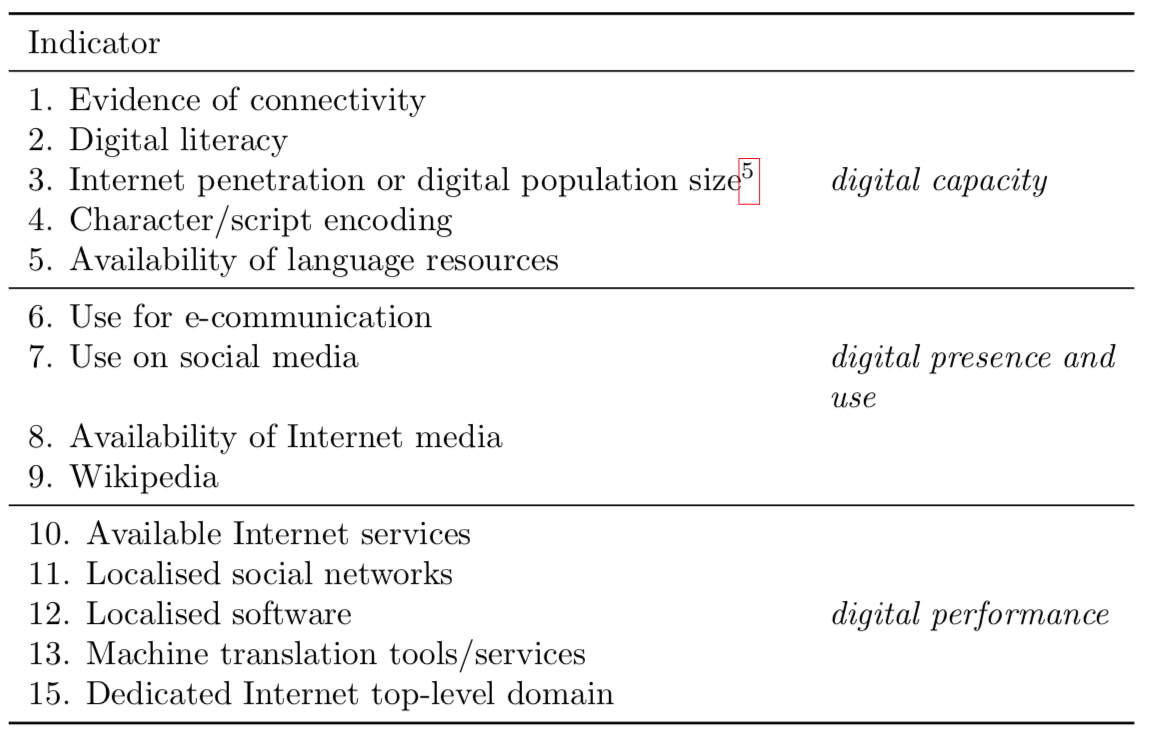
\includegraphics[width=.8\textwidth]{img/dldp.png}
 \caption{Indicators of digital vitality \citep[6]{soria2017digital}}
 \label{fig:dldp}
\end{figure}

Soria et al. go into depth about each of these factors. As an example, for localised software, they propose the following scale in Table~\ref{table:dldp-software}. They explain, for each scale, how to find information - for instance, they suggest asking local researchers and community members about the usage of "Windows, Mac OS X, Linux, Android, iOS, Microsoft Office, LibreOffice, Firefox, Chrome, Internet Explorer, Thunderbird, Adobe Creative Suite, Gimp" for judging localised software. However, they do not show metrics on any languages judged according to this scale, and they don't make it clear whether or not the different metrics ought to be summed to come up with a single number (an issue which \citet{lee2016assessing} raised with the UNESCO rating). In conclusion, while this is an interesting and in-depth metric, its wider applicability is not clear.

\begin{table}
\begin{center}
\begin{tabular}{|p{2cm}|p{1cm}|p{10cm}|} \hline
Label & Grade & Localised software \\ \hline
none & 2 & Neither operating system nor general purpose soft- ware localised in the language\\
limited & 3 & At least one operating system (either desktop or mo- bile, either open or commercial) localised in the language \\
medium & 4 & At least one desktop and one mobile operating system (either open or commercial) + some general purpose software (a word processor and a browser) localised in the language\\
strong & 5 & Most used operating systems and general purpose software localised in the language; some specific purpose application software localised.\\
advanced & 6 & Main operating systems and application software localised in the language.  \\ \hline
\end{tabular}
\end{center}
\caption{Scale for Localised Software}
\label{table:dldp-software}
\end{table}

Each of these metrics suffers from growing pains. For instance, there is no metric as of yet which ranks English in it's own category - something which was seen as a large enough issue to cause the EGIDS authors to add another 0 ranking for supranational languages. (TODO: Write a paper on this) As well, there hasn't been an integrated approach looking at quantitative and qualitative measurements together. The most substantial work on this has been Kornai's team, which has worked with funding from SIL International on a Digital Language Vitality database\footnote{\href{https://hlt.bme.hu/en/projects/lingvit}{https://hlt.bme.hu/en/projects/lingvit}}. However, the future for this work as, at this moment, unclear (Kornai in personal communications, 2018).

% There's no higher scale - what separates English from French?
% What about coding _in_ a language? How many languages have native computer languages?

\subsubsection{BLARK and LREMaps}

\citet{soria2017digital} briefly mention "digital language survival kits" as one of the motivations for their paper - these are explicated more fully on the Digital Language Diversity Project's site.\footnote{\href{http://www.dldp.eu/en/content/digital-language-survival-kit}{http://www.dldp.eu/en/content/digital-language-survival-kit}} This project is an EU initiative, through the Erasmus+ programme, and it aims to identify needs and provide "kits" for certain European low resource languages - specifically Basque, Breton, Karelian and Sardinian.

The use of the word kit is informative, as there is pre-existing literature on this topic in BLARK, or Basic Language Resource Kit, developed by ELSNET, a European international umbrella for 145 different organisations in 29 countries, and first outlined in 1998 \citep{krauwer2003basic}. The BLARK is defined as the "minimal set of language reosources that is necessary to do any precompetitive research and education at all." \citep[4]{krauwer2003basic} In general, this comprises "written language corpora, spoken language corpora, mono- and bilingual dictionaries, terminology collections, grammars, modules (e.g. taggers, morphological analysers, parsers, speech recognisers, text-to-speech), annotation standards and tools, corpus exploration and exploitation tools, bilingual corpora, etc." The initial paper offered by \citet{krauwer2003basic} describing BLARK itself has a comprehensive matrix in the appendix outlining technology that would be needed to provide a BLARK for Dutch, as outlined in a workshop documented in \citet{binnenpoorte2002towards}. In another paper, \citet{maegaard2006blark} under NEMLAR (Network  for  Euro-Mediterranean  LAnguage  Resources) outlined the specific needs that BLARK specified which could be applied to Arabic, and actions which researchers took in order to develop resources to best fill in the grid. The BLARK process - auditing a language, using a grid to identify what corpus and resource needs are necessary for language resources - has now been applied to Swedish \citep{elenius2008language} and Bulgarian \citep{simov2004language}, and numerous South African languages \citep{grover2011south}, among others.

Unfortunately, BLARK (or ELARK, purportedly a more sophisticated version of BLARK for industry described in \citet{mapelli2003report}, according to \citep{grover2011south}) is a large grid, and may not work for languages without extensive funding models or support. For this, there is a smaller BLARK version, the BLARKette, which should work for low resource languages.

\begin{quote}
In order to accommodate this problem we have proposed the definition of a scaled down, entry-level version of the BLARK, targeting exclusively the research and (especially) the education community. It should be light and compact, not too demanding in terms of hard and software requirements, cheap, free from IPR issues, and ideally small enough to fit on a CD or DVD. We expect to release a first document, with tentative summary specifications, towards the end of 2006. Check the ELSNET site for news. \citep{krauwer2006strengthening}
\end{quote}

The model of transportation for this - a CD, instead of a downloadable resource - shows that the concept has not aged well. There is a also surfeit of references of BLARK or BLARKette in the past decade in the literature. What happened? It is most likely (but not backed up by proof) that building BLARK is too difficult task to perform and lacks proper incentives. It requires an authoritative and intimate knowledge of a language's space by many researchers, all of whom must come together to identify gaps, often from proprietary institutions. This is a difficult task.

But this, in some sense, has expanded into LRE (Language Resources and Evaluation) maps, within Europe. As described in \citet{calzolari2010lrec, del2014lremap, mariani2015language, del2015visualising}, the Language Resources and Computation %TODO
conference organisers began asking authors to fill out basic language resource grids when submitting papers. This data has been collected into matrices and a database that reflects language resources for a variety of languages. To date, this is the most comprehensive review of NLP per language that I'm aware of - however, it's worth noting that it is limited in scope. The 133 less-common languages represented in the LREMap represent only 414 entries. An example of the matrix for the high resource languages can be seen in Figure~\ref{fig:lre}.

\begin{figure}
 \centering
 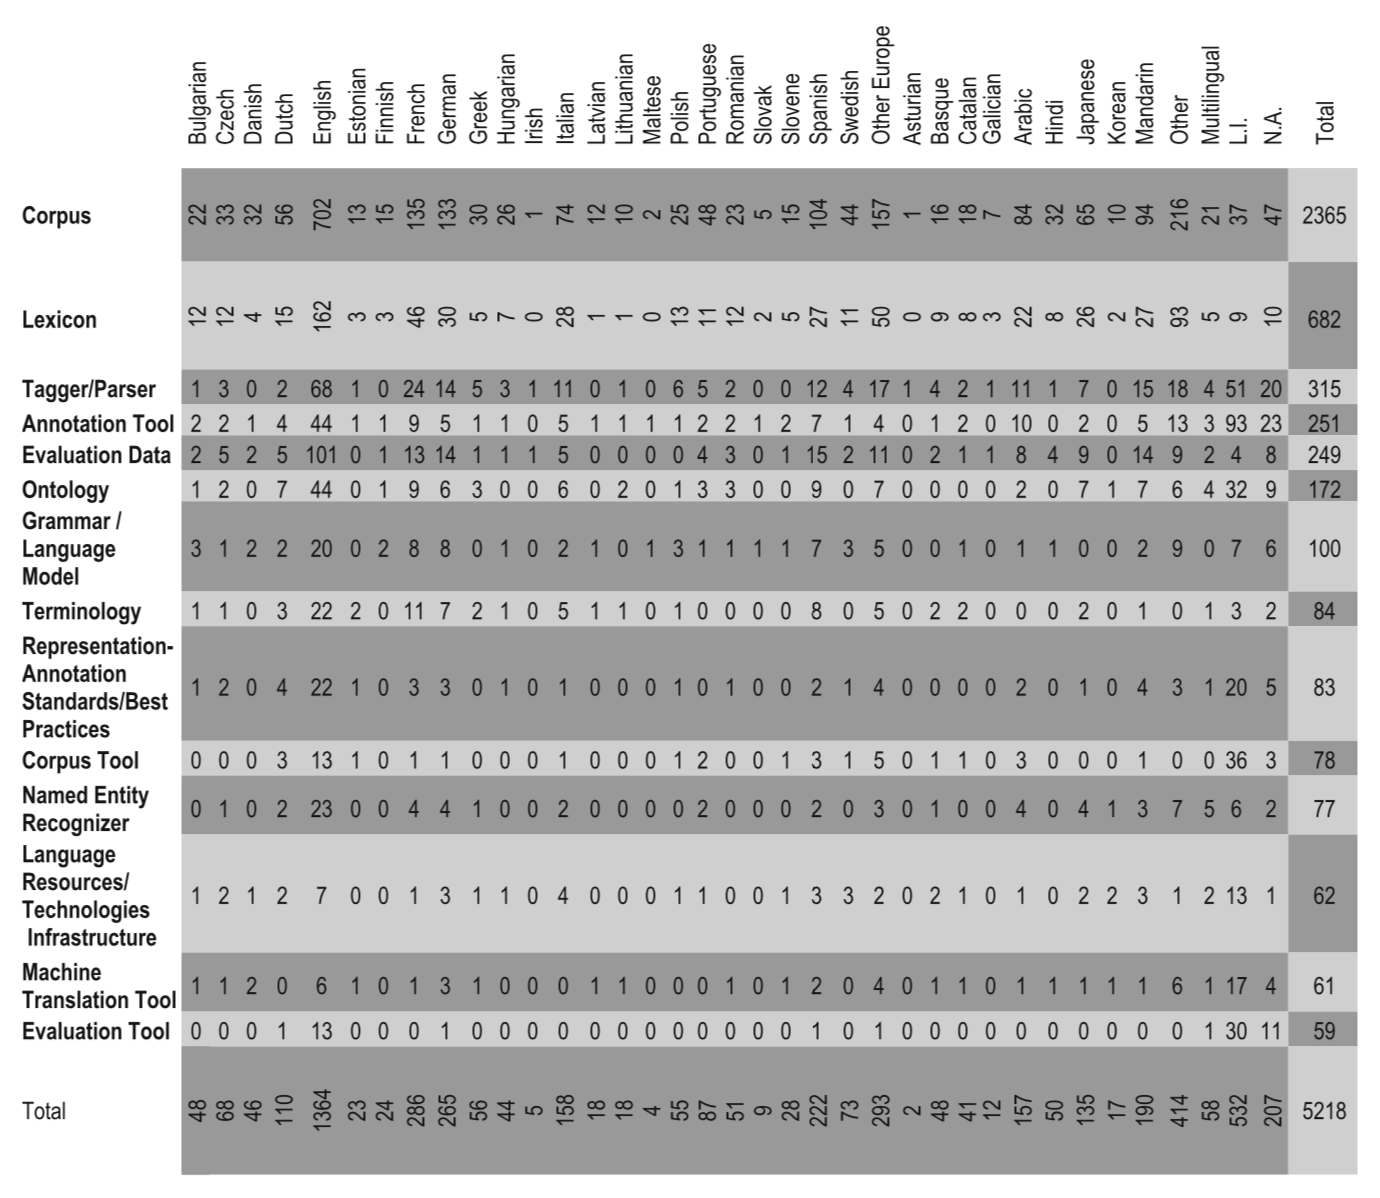
\includegraphics[width=.8\textwidth]{img/lre.png}
 \caption{LRE maps for high resource languages \citep[460]{mariani2015language}}
 \label{fig:lre}
\end{figure}

Several coauthors working on the LRE maps research are also coauthors of the \citet{soria2017digital} paper; extending the LRE maps for low resource languages, and then intensifying efforts to develop low-hanging fruit for low resource languages is a logical next step for this research. The focus on European languages is expected; this may stem from the fact that LREC, the main conference series from which LRE data was drawn, is run by the European Language Research Association (ELRA). This fragmentation of the field is to be expected, and happens in the reverse, as well: for example, \citet{paricio2010new} cites a framework for upgrading low resource languages which is explained in a research paper written in Spanish, and half of the papers presented at the Ryukyuan Heritage Language Society's conference in Tokyo in 2012 (which I attended) were presented in Japanese. This is not to say that fragmentation and diversity of linguistics in academia is something to be avoided, but rather that it is a hurdle to be noted and worked with to avoid repeated work and splintered efforts.

%\subsection{The current state of language diversity}
%
%In this section, I am going to briefly go into detail about what diversity means for linguistics. This will be useful later for explaining how related languages can be used to bootstrap work in similar languages. For instance, Irish spell-checkers and constitutional corpora from the EU can be used by Scottish Gaelic speakers with some tweaks in order to further improve their own systems.
%

\subsection{Who makes resources for languages?}
Another hurdle which was briefly alluded to earlier was the plethora of large organisations, databases, or projects dedicated to cataloguing low resource languages. Each of these has differences in scope, funding, and incentives. However, large organisations are not the only groups working on language development, digital ascent, language revitalisation, or any other shared focus that relates to low resource languages.

As \citet{hammarstrom2015unesco} points out, "language documentation and description is an extremely decentralized activity, carried out by missionaries, anthropologists, travellers, naturalists, amateurs, colonial officials, ethnographers and not least linguists over several hundred years." Language communities, amateur and professional linguists, educators, and language policy setters are most often involved in standardising a language and helping to document and revitalise low resource languages. Digitally, amateur computational linguists, and coders who are first language speakers of their own language are often the first to work on translating or migrating resources; this group is also often the first to set up Wikipedias in a local language (although this often leads to enthusiastic loners working outside of the main language communities) \citet{soria2017digital}. Beyond these groups, universities, local governments and businesses can also often develop language resources for low resource languages, as was the case with \citet{rognvaldsson2009icelandic}. After these groups, large grant-driven institutions such as CLARIN or the NSF fund a large portion of language development, along with industry giants such as Google or Xerox, and large military research arms such as DARPA.

Unfortunately, the lion's share of the overall funding for language development goes to languages which are already resourced.

\begin{quote}
Over the years the EU has invested massively in the development of language and speech technology, and many dedicated R\&D programmes have had a significant impact on its advancement, including applications oriented towards solving the multilinguality problem... Unfortunately the strong industrial bias of recent EU programmes has led to a situation where the major part of the funding for language and speech technology goes to the major languages. This is not surprising, as industrial players will prefer to invest in the development and deployment of technologies for larger markets. As a consequence there has been only marginal support for the development of language and speech technology for the language communities that do not constitute profitable markets. As the development cost of such technologies is independent of the number of speakers of a language ("all languages are equally difficult") this has created a very unbalanced situation. \citep{krauwer2006strengthening}
\end{quote}

Or:

\begin{quote}
Were it not for the special attention DARPA, one of the main sponsors of machine translation, devoted to Haitian Creole, it is dubious we would have any MT aimed at this language. There is no reason whatsoever to suppose the Haitian government would have, or even could have, sponsored a similar effort \citep{spice}. \citep[9]{kornai2013digital}
\end{quote}

Another good example of where funding and incentives for language development can be controversial would be Ethnologue, which rate limits and has a paywall guarding usage of their database, even though they are widely recognised as one of the best informed databases for language data. SIL International also gatekeeps the standard ISO 639-3, which is the most widely used language code. By having a paywall on their data, they exclude the general public from having control of codes for their own languages. SIL has also come under criticism for their Christian missionary work, as it can be viewed as complicit in culture change, and by extrapolation, ethnocide \citep{dobrin2009sil, dobrin2009practical, everett2009don}. This is just one example - and most likely one of the most extreme, not counting military work on languages used by insurgents in wars - of how organisations working on language resources may influence the work itself.

The funding of language resource development matters, because the way that the language community approaches language development affects the chance of survival for the language. This is one of the reasons that \citet{grenoble2016response} pointed out that "language vitality" is a more politically correct term to use than "language endangerment", as it takes the focus away from loss and focuses attention on language ascent. Another reason that language funding matters is because the major players with funding will generally be able to out manoeuvre smaller groups with different resources. This can enforce language shift, and can render resources created by individual developers moot. For instance, the secwepemc-facebook\footnote{\href{https://github.com/kscanne/secwepemc-facebook}{https://github.com/kscanne/secwepemc-facebook}} tool developed to automatically translate Facebook into low resource languages, created by the developer Neskie Manuel for his native Secwepemcts\'in, is no longer an active project and has not been updated, rendering it obsolete with Facebook UI changes, while automatic translation is provided for high resource languages natively by Facebook. Scannell, who helped port the secwepemc-facebook tool to Greasemonkey, was one of the authors of \citet{streiter2006implementing}, which suggested that developers for low resource languages use open source software pools in order to pool resources to enable them to overcome this - among other - issues facing low resource languages in particular.

As in Section~\ref{subsubsec:response}, covering all of the potential issues with funding and the politics of language development is well beyond the scope of this paper. However, focusing on how open source can help low resource languages is not. But first; what do I mean by "open source"?

% Here, I will explain briefly who makes language resources for these languages. I'll explain what I see as the main groups doing this work: professional translators, educators, missionaries (of multiple faiths, but mostly Christian), academics and native technologists. I'll explain each stakeholder and their canonical perspectives.

% Alexis: what do you mean by "their canonical perspectives"? will this section address creation of digital resources only, or all resources? for that matter, what counts as a digital resource? does a collection of pdf scans of old books count? how about a pdf version of a text collection? etc....
% I don't immediately see how this fits into the rest of the thesis. also look at relevant publications from Jeff Good - one in particular on the ecology of language documentation: http://www.acsu.buffalo.edu/~jcgood/publications.html


%\subsection{Language research funding}
%
%Here, I'll go into more depth about funding, as we've outlined who works on LRLs and who would fund research, and why. This will further inform the basis for the work of the previous section. I'll talk about DARPA MT funding in the 20th century, as well as other efforts such as CLARIN.



% IARPA and DARPA both are involved with low resource languages and both of them may have their own institutional values that are probably at ends with independent researchers, commercial consumers, and language communities. Does working on sparse data openly bring along with it ethical or moral concerns; if so, how can these be adequately explained, breached, and talked about? How can they be worked around or be part of the conversation? Note that DARPA and the like also use humanitarian reasons as their primary stated aim for work on sparse languages, which may be contrary to their military needs. There is already an extensive literature on moral uses of data -- I could summarize that, and apply it specifically to low resource languages, which is something I do not think has yet been published.

% Darpa: http://www.darpa.mil/program/low-resource-languages-for-emergent-incidents
% IARPA: http://www.iarpa.gov/index.php/research-programs/babel

% - Institutional bottleneck
% - Linguistic colonialism
% - Ethical and moral concerns for military usage
% - Ethical and moral concerns for big business usage


% The State of endangered languages and computational linguistics
%\subsection{Definining Endangered Languages}
%\subsection{What are computational resources}
% !TEX root = thesis.tex
\section{Open Source Code}
\label{sec:open-source}

% Changing tack, here I will talk about what \emph{open source} means. This is important - otherwise, this thesis is just a rehash of current existing computational work on LRLs.

\subsection{Defining {\it Open Source}}
\label{subsec:defining-open-source}

{\it Open Source} is a complex term which refers to any code, not just code related to computational linguistics. Here, I'll define what I mean by Open Source. This will largely inform the next section where I talk about its use for low resource languages.

At its core, {\it open source} refers to code which has a license which allows it to be available to freely inspect, use, or modify by anyone. It was introduced in 1998 by Linux programmers such as Eric Raymond, author of {\it The Cathedral and the Bazaar}\footnote{\href{http://www.catb.org/~esr/writings/cathedral-bazaar}{http://www.catb.org/~esr/writings/cathedral-bazaar}}\citep{raymond1999cathedral}; Linus Torvalds, author of the Linux kernel\footnote{\href{https://www.kernel.org/}{https://www.kernel.org/}} and Git\footnote{\href{https://git-scm.com/}{https://git-scm.com/}}; Richard Stallman, founder of the GNU project\footnote{\href{https://www.gnu.org/}{https://www.gnu.org/}} and the Free Software Foundation\footnote{\href{https://www.fsf.org/}{https://www.fsf.org/}}; and others in response to the Netscape browser's code being openly licensed and made available.

{\it Open source} is one of many terms which can be used to differentiate code which is either available or licensed permissively for re-use; other terms include {\it free} and {\it libre} software. There is no standard definition of open source that is universally accepted.

Nor will universal acceptance be forthcoming. The issue regarding reconciliation between open source, free software, and the rest of the terms stems largely from a difference of opinion between what constitutes open software, and what free and open means. An oft-used expression is "free as in beer"as opposed to "free as in speech", where the first is used for gratis software which has no monetary price set on it, as opposed to software which is written without restriction. The term {\it libre} is most often used for the second, to differentiate the two meanings in English. Occasionally, the acronym FLOSS is used in open source parlance to refer to Free Libre Open Source Software, which is both gratis and libre software.

For some adherents, software ought to be free (gratis), as it is a result of human labour and because opening it up without cost maximises the utility function of that code, and minimises duplicated effort. This idea contains within it the seed of the digital commons: like the commons in philosophical and economic literature, code can be viewed as a resource that belongs to humanity as a whole, and not the creators who initially fashioned it. In this sense, open source is a more of a philosophical theme than a technical term.

\begin{quote}
Open source is a development methodology; free software is a social movement. For the free software movement, free software is an ethical imperative, essential respect for the users' freedom. By contrast, the philosophy of open source considers issues in terms of how to make software  "better" - in a practical sense only. It says that nonfree software is an inferior solution to the practical problem at hand.\footnote{\href{https://www.gnu.org/philosophy/open-source-misses-the-point.html}{https://www.gnu.org/philosophy/open-source-misses-the-point.html}}
\signed Richard Stallman (Founder of GNU\/Linux)
\end{quote}

However, for the most part, "open source" isn't disambiguated as a term, because authority for this task is relegated to the license put on a piece of software, which determines the legality and potential use. Licenses determine the legal rights to sharing code. A piece of code which is taken from a proprietary server and published on the internet is not necessarily open source. In this instance, the code may have been illegally copied and shared, but it is not licensed for free usage. Under no definitions is this considered open source. Indeed, this touches upon issues of digital copytheft and "piracy", which is a standard term used frequently in the media and in legal proceedings to attach a sense that copying code is the same as larceny or theft on the high seas. Avoiding the question of the validity of this viewpoint, it is important to focus on the license as the differentiating factor between code which has been released legally under an "open" definition or not. The term 'open source' under most definitions doesn't pertain to ethical concerns about the software's usage, but rather simply refers to whether or not it is permissively licensed and available for users.

For that matter, work published without a license on a public repository site, such as on GitHub\footnote{\href{https://github.com}{https://github.com}}, is not technically open source, either. When software is not licensed, it by default reverts to copyright where{\it all rights are reserved}, which is by definition not FLOSS. For this reason, it's important to add a license to code if it is in your purview to do so, and if you wish to follow the open source methodology. There are many licenses which are considered to be open source, and there are several arbiters available which judge the validity of open source licensing. The Open Source Initiative maintains a list of approved licenses on their website\footnote{\href{https://opensource.org/licenses}{https://opensource.org/licenses}}.

The Open Source Institute (OSI), whose founders were one of the original coiners of the term {\it open source}, has several parameters by which open source software can be judge as being 'open' or 'closed' (that is, proprietary, non-permissively licensed, non-reusable, limited in usage to a set amount of people, and so on). It may be useful to list these terms directly below, as they are instructive about how open source can be a nuanced term. These terms and their definitions are from the OSI's website \footnote{\href{https://opensource.org/osd}{https://opensource.org/osd}}, and are repeated below verbatim.

\begin{enumerate}
\item{Free Redistribution}. The license shall not restrict any party from selling or giving away the software as a component of an aggregate software distribution containing programs from several different sources. The license shall not require a royalty or other fee for such sale.
\item{Source Code}. The program must include source code, and must allow distribution in source code as well as compiled form. Where some form of a product is not distributed with source code, there must be a well-publicized means of obtaining the source code for no more than a reasonable reproduction cost, preferably downloading via the Internet without charge. The source code must be the preferred form in which a programmer would modify the program. Deliberately obfuscated source code is not allowed. Intermediate forms such as the output of a preprocessor or translator are not allowed.
\item{Derived Works}. The license must allow modifications and derived works, and must allow them to be distributed under the same terms as the license of the original software.
\item{Integrity of The Author's Source Code}.
  The license may restrict source-code from being distributed in modified form only if the license allows the distribution of "patch files" with the source code for the purpose of modifying the program at build time. The license must explicitly permit distribution of software built from modified source code. The license may require derived works to carry a different name or version number from the original software.
\item{No Discrimination Against Persons or Groups}.
  The license must not discriminate against any person or group of persons.
\item{No Discrimination Against Fields of Endeavor}.
  The license must not restrict anyone from making use of the program in a specific field of endeavor. For example, it may not restrict the program from being used in a business, or from being used for genetic research.
\item{Distribution of License}.
  The rights attached to the program must apply to all to whom the program is redistributed without the need for execution of an additional license by those parties.
\item{License Must Not Be Specific to a Product}.
  The rights attached to the program must not depend on the program's being part of a particular software distribution. If the program is extracted from that distribution and used or distributed within the terms of the program's license, all parties to whom the program is redistributed should have the same rights as those that are granted in conjunction with the original software distribution.
\item{License Must Not Restrict Other Software}.
  The license must not place restrictions on other software that is distributed along with the licensed software. For example, the license must not insist that all other programs distributed on the same medium must be open-source software.
\item{License Must Be Technology-Neutral}.
  No provision of the license may be predicated on any individual technology or style of interface.
\end{enumerate}

\subsubsection{Open Source Licenses}
\label{subsec:licenses}

These different terms and conditions are often conflated, and a legally-valid license which satisfies all of them is difficult to write on an {\it ad hoc} basis. For this reason most open source programming relies on using existing licenses, and copying them for specific projects. There are tools today to help make licensing more clear to na�ve users, such as \href{https://choosealicense.com}{choosealicense.com}, \href{https://tldrlegal.com}{tldrlegal.com}, and so on.

Some of the main licenses used in the wild are as follows:

\begin{itemize}
\item The MIT license, developed at MIT, is the most popular license on GitHub, the world's largest repository of code, used in over 40\% of the projects licensed there as of March 2015.\footnote{\href{https://blog.github.com/2015-03-09-open-source-license-usage-on-github-com/}{https://blog.github.com/2015-03-09-open-source-license-usage-on-github-com/}} It is a a very permissive license, which allows commercial use, modification, distribution, sublicensing, and private use of any code so licensed. It also waives liability for the authors of the code, saving them from needing to worry about lawsuits in cases where their code would otherwise be liable - the code is granted as is, and what the user does with it is not the author's fault. The only restriction is that you need to include the license in any software which uses it.
\item The Apache License 2.0, developed by the Apache Software Foundation\footnote{\href{https://www.apache.org/licenses/}{https://www.apache.org/licenses/}}, is similar, but disallows users from trademarking code with the license, requires a few smaller modifications like stating code changes and adding a NOTICE file, if one exists, to derivational code, and also adds a patents clause for contributors.
\item The BSD licenses were developed for use with Berkeley Software Distribution, a Unix-like OS. There have been multiple iterations; the first, 4-clause license required every subsequent license to reference and acknowledge the original, ending with large lists of acknowledgements; a subsequent 3-clause license (often called the "New" BSD) removed this, but kept a clause which stated that usage does not imply endorsement by the original contributors; and this was removed in a 2-clause version, often called "Simplified" or the "FreeBSD" license. 
\item The GNU General Public License (GPL)\footnote{\href{https://www.gnu.org/licenses/}{https://www.gnu.org/licenses/}} is the main example of copyleft licensing, where any derivative works that use GPL licensed code must also use a GPL license. This causes major issues when users want to combine code from multiple sources, some of whose licenses may conflict. For this reason, the GNU Library or "Lesser" General Public License (LGPL) was created, to allow only code under the LGPL to be accessible and modifiable openly, while all other code doesn't have to be. GPL also demands that users include installation instructions, 
\item Creative Commons licenses\footnote{\href{https://creativecommons.org/licenses/}{https://creativecommons.org/licenses/}}, mostly used for sharing non-code material such as images and documents openly, was created by Lawrence Lessig, the founder of the Creative Commons organisation\footnote{\href{https://creativecommons.org/}{https://creativecommons.org/}}, and may also be used for code projects. There are many licenses they offer, and some variants are copyleft licenses - in particular, "share-alike" clauses are an example of copyleft. 
\item The Unlicense\footnote{\href{https://unlicense.org/}{https://unlicense.org/}}, created in 2010, is another option, which explicitly states that code is unlicensed, with no restrictions, and also with no liability for the authors (unlike code which is not licensed, which has stricter protections under US copyright law than code which specifically excludes a license). There is a Creative Commons Zero\footnote{\href{https://creativecommons.org/publicdomain/zero/1.0/}{https://creativecommons.org/publicdomain/zero/1.0/}} license which is similar, as well as the WTFPL license ("Do What The Fuck You Want Public License")\footnote{\href{http://www.wtfpl.net}{http://www.wtfpl.net}}, which, although intentionally comically profane, is non-trivial in that it is used in 11,714 different software projects on GitHub as of this writing.\footnote{\href{https://github.com/search?q=license\%3AWTFPL}{https://github.com/search?q=license\%3AWTFPL}} 
\end{itemize}

Ultimately, licenses are complicated legal documents with various repercussions for how code is accessible. 

\subsection{Where is open source code?}
\label{subsec:where-is-open-source-code}

For closed source or proprietary software, the code itself often isn't stored in the open or accessible to third parties. However, for open source software to be defined as open source according to OSI's definitions, it needs to be publicly accessible and well-publicised. This means that storing code on a server where it could technically be accessed via some protocol, or less ideally through a mail-order CD as \citet{krauwer2006strengthening} suggested, is not enough; instead, it ought to be linked to elsewhere and available for everyone to access. This raises the question: where is most open source code stored? 

Unequivocally, GitHub\footnote{\href{https://github.com}{https://github.com}} is the largest source of shared, open code on the internet, with 27 million users and 80 million repositories as of March 2018\footnote{\href{https://github.com/about}{https://github.com/about}}. There have been several large-scale studies of its codebase by researchers \citep{gousios2012ghtorrent, allamanis2013mining, gousios2014lean, kalliamvakou2014promises, beller2016analyzing} which confirm this. Other large repositories for code of a similar nature, include Sourceforge, with 430k projects and 3.7m users\footnote{\href{https://sourceforge.net/}{https://sourceforge.net, accessed April 18, 2018}}, Bitbucket\footnote{\href{https://bitbucket.org/}{https://bitbucket.org/}} with 5m users\footnote{\href{https://blog.bitbucket.org/2016/09/07/bitbucket-cloud-5-million-developers-900000-teams/}{https://blog.bitbucket.org/2016/09/07/bitbucket-cloud-5-million-developers-900000-teams/}},  Launchpad\footnote{\href{https://launchpad.net/}{https://launchpad.net/}} with 4.2m users\footnote{\href{https://launchpad.net/people}{https://launchpad.net/people}}, and Gitlab\footnote{\href{http://gitlab.com/}{http://gitlab.com/}}, which holds the majority share of self-hosted Git platforms\footnote{\href{https://about.gitlab.com/is-it-any-good/}{https://about.gitlab.com/is-it-any-good/}}. All of these platforms are based around Git, the versioning software developed by Linus Torvalds, used to store different versions of code for developers and teams, which lends itself particularly to shared code that can be updated easily by outside and community developers. It is worth mentioning that not all of these projects are public. 

Self-hosted Git instances are a common way of storing proprietary code; one sets up a versioning system within a company, using the tools and set of social standards that developers are used to from working on open source code, but limit access to employees. This is what is meant by GitLab's statement that they host most self-hosted Git platforms. Git isn't the only possible versioning software for this; Google has their own versioning tool, Piper, which hosts the over two billion lines of code used by the majority of the company.\footnote{\href{https://www.wired.com/2015/09/google-2-billion-lines-codeand-one-place/}{https://www.wired.com/2015/09/google-2-billion-lines-codeand-one-place/}} Self-hosted Git instances are generally not open source - generally, one is limited to a hosting service such as GitHub, where one pays a fee for hosting, or, more commonly today, hosts for free if public, but pays a fee for private hosting. 

There are alternatives to cloud storage (the cloud here being a common metaphor for hosting on someone else's servers) with a hosting provider; one would be storing the code on one's own website, and running your own server or building the user interface yourself. This is largely uncommon due to setup costs, but occasionally happens with academics and smaller teams who are not used to larger hosts or who are worried about the longevity of providers. This latter worry is founded; for instance, Google Code was closed after ten years of running in 2016, causing many projects to need to port to another service such as GitHub.\footnote{\href{https://code.google.com/}{https://code.google.com/}} For academics, a common solution to offset setup and hosting costs is to use university websites and archives as a suitable place to store open source code. For instance, Giellatekno, a language-technology research group, and Divvun, a linked product development group, both work primarily on S�mi languages, and both use the same Subversion (another versioning system) database for storing their code \citep{moshagenopen}, which is hosted by UiT The Arctic University of Norway.\footnote{\href{http://giellatekno.uit.no/}{http://giellatekno.uit.no/}} 

In a large part, the question of where to store information is one which the large archival sites mentioned in Section~\ref{subsec:finding-resources} was made to solve. In particular, this is true for non-code resources, such as audio and video corpora, which historically have prioritised for storage over code due to the size of the corpora and due to the older industry standards of keeping all code related to research private, especially when that code was funding by enterprise. Many of these sites were repositories of metadata which pointed to individually hosted content, which made the links susceptible to link rot and offloaded the issue of storage altogether. 

Today, however, there is a sea change towards putting computational work in the open. Occasionally, this means that academics point to the open source code for their papers on GitHub or elsewhere, or publish their software itself as a research object. For example, \citet{makela2016integrated} and \citet{kleinberg2017web} were published with the Journal of Open Source Software (JOSS)\footnote{\href{http://joss.theoj.org/}{http://joss.theoj.org/}}, which peer-reviews, publishes, and assigns digital object identifiers (DOIs) to software as a way of recognising important academic work. The code for these papers is publicly available on GitHub. 

\subsection{Digital Permanence and Storage}
\label{subsec:digital-permanence}

Universities and institutions have short timelines and are largely dependent on specific, allocated, and thus finite funding. Here, I'll answer the question: What other models are there for data storage? What concerns are there?

% Alexis: there are also issues around evolution of code -- what about open source code that does great things but requires, e.g., java from 10 years ago?

\subsection{Data and privacy}
\label{subsec:data-and-privacy}

Here, I'll talk specifically about data rights and privacy, in regards to whether it makes sense to decouple code from data, especially in cases of low resource languages, where sparse data may be naturally enriched with annotation schemas and hard to separate out from the tools being used. In such cases, how do we as a community, researchers as providers, and developers as consumers, deal with licensing, privacy, and proprietary data? Does it make sense to provide links to code that can be used institutionally or commercially without also allowing for things like royalties for usage, or proper licensing for data? Bound up in this are also ethical concerns - well studied in theoretical field linguistics - about the language users themselves not wishing for their data to be used in certain ways.

% From Chiarcos:

% a few years back, I compiled a massive corpus of Bibles and related texts
%in a CES-conformant XML format (following Resnik 1996), some also with
%annotations. For the most part, distributing this corpus would be illegal
%under European copyright law (and that's why you haven't heard about it),
%but I realized that there are circumstances which could allow
%dissemination of a great part of it under an academic license.

% Compiling and distributing a web corpus is basically illegal in Europe
%unless explicitly permitted by an accompanying license. However, US law
%has the concept of fair use, and if a data provider declares US
%legislation to apply (e.g., that "[t]hese Terms and Conditions ... are
%governed by the laws of the State of New York"), we Europeans can rely on
%the principle of fair use, as well.
%
%% According to 17 U.S.C. § 107, "the fair use of a copyrighted work,
%including such use by reproduction in copies or phonorecords or by any
%other means specified by that section, for purposes such as criticism,
%comment, news reporting, teaching (including multiple copies for classroom
%use), scholarship, or research, is not an infringement of copyright." The
%intended use is for NLP research, DH scholarship and classroom use, so
%that would probably not an issue -- and in fact, there is no financial
%damage whatsoever as this data is freely and redundantly available from
%the web.
%
%% However, am I allowed to distribute this corpus with an explicit license
%statement? I think CC-BY-NC should protect the intellectual and commercial
%interests of the creator of the electronic edition and be roughly in the
%spirit of an academic license, but of course, I'm not the actual owner of
%the data, but only responsible for its transformation and annotation. I am
%wondering about the consequences if someone eventually creates an NLP tool
%chain from this data and uses any models trained on the data in a
%commercial application. As the original copyright extends to derived
%works, this would be a clear violation of my license statement, of course,
%but I would be responsible as I redistributed the data and by transforming
%it from messy HTML to proper markup, I actually enabled this violation.


\subsection{Legal rights and liability}
\label{subsec:legal-rights}

Here, I'll talk about specific licenses used in Open Source, and how they apply to code. I'll try to keep this brief.

I'll also talk about liability wavers - a separate issue from licenses. I'll talk about the standard liability wavers used with the MIT license, and other issues that might arise for language code specifically.

\subsection{Military and enterprise solutions}
\label{subsec:military-and-enterprise}

In this section, I will talk about how open source meshes with military and enterprise development.

%% https://www.nist.gov/itl/iad/mig/lorehlt-evaluations, DARPA

\subsection{Funding}
\label{subsec:oss-funding}

Here, I'll talk about funding again - but in terms of open source code. This will be a short section.

% IARPA and DARPA both are involved with low resource languages and both of them may have their own institutional values that are probably at ends with independent researchers, commercial consumers, and language communities. Does working on sparse data openly bring along with it ethical or moral concerns; if so, how can these be adequately explained, breached, and talked about? How can they be worked around or be part of the conversation? Note that DARPA and the like also use humanitarian reasons as their primary stated aim for work on sparse languages, which may be contrary to their military needs. There is already an extensive literature on moral uses of data -- I could summarize that, and apply it specifically to low resource languages, which is something I do not think has yet been published.

% Darpa: http://www.darpa.mil/program/low-resource-languages-for-emergent-incidents
% IARPA: http://www.iarpa.gov/index.php/research-programs/babel

% - Institutional bottleneck
% - Linguistic colonialism
% - Ethical and moral concerns for military usage
% - Ethical and moral concerns for big business usage

\subsection{Ethical reasons for using open source}
\label{subsec:oss-ethics}

Finally, I want to close with a discussion of the moral and ethical reasons for using open source, and whether or not these concerns are relevant to computational linguists.

% \subsection{Defining "open source"}
% \subsection{Where is open source code?}
% \subsection{Data rights and privacy}
% \subsection{Liability}
% \subsection{Funding}
% \subsection{Military and enterprise solutions}
% \subsection{Ethical reasons for using open source}
% !TEX root = thesis.tex
\section{Open Source Code for Low Resource Languages}\label{sec:endlangcode}
% Open Source code for endangered languages

In this section, I'll move on to the real meat of this thesis; how is open source code used for computational linguistics, and specifically for LRLs.

\subsection{BLARK and beyond}

First, I am going to talk about BLARK - the Basic LAnguage Resource Kit proposed by \citet{krauwer2003basic} - and what a language needs digitally as a base layer to digitally ascend. I haven't talked specifically about how computational linguistics addresses low resource languages yet - the preceding sections have largely been showing the state of the field and what open source is. We'll get to open source eventually, but here I want to cover the tools needed for a language.

I'll then mention tools here that can be used after a language has some digital presence - basically, what makes an LRL a resourced language.

%% http://www.blark.org/
%% Blark:  The BLARK concept was defined in a joint initiative between ELSNET (European Network of Excellence in Language and Speech) and ELRA (European Language Resources Association) [Krauwer, 1998] and first launched with a Dutch initiative called Dutch Human Language Technologies Platform that was initiated in April 1999. Then, in the framework of the ENABLER thematic network (European National Activities for Basic Language Resources -Action Line: IST-2000-3.5.1), ELDA elaborated a report defining a (minimal) set of LRs to be made available for as many languages as possible and mapping the actual gaps that should be filled in so as to meet the needs of the HLT field.

%% http://www.elsnet.org/dox/blark.html

%% Quote some BLARK papers from various languages - relatively easy to find papers.


\subsection{NLTK and other open source libraries}

Here, I'll explain some open source resources that can be used to bootstrap development; for instance, \href{NLTK (Natural Language Toolkit)}{http://nltk.org/}, a free and open source library which uses the Python language by \citet{bird2006nltk}, and enables users to interface with over fifty different corpora and lexical resources.

% A primer written by the main creators, \href{Natural Language Processing with Python}(http://nltk.org/book), is used frequently in natural language processing classes written by the creators. It is licensed under the Apache 2.0 license, a common license \footnote{https://github.com/nltk/nltk/blob/develop/LICENSE.txt}. On GitHub, there are currently 204 contributors listed \href{https://github.com/nltk/nltk/graphs/contributors}, although the git history shows 234 (found by using the command `git authors` % TODO Explain
% ). Some of the resources within NLTK have to do with low resource languages. For instance, in 2015, NLTK added machine translation libraries, including popular ones such as IBM Models 1-3 and BLEU.

% By open sourcing their code, the NLTK authors have allowed it to be adapted and re-used. Currently, there are several ports.
% % TODO cite.
% One of these is the JavaScript language implementation, \href{https://github.com/NaturalNode/natural}{https://github.com/NaturalNode/natural}. This has 6700 stars on GitHub, which is a good indicator of community vitality and use, and 88 contributors. The port is also open source, under an MIT license \href{https://github.com/NaturalNode/natural\#license}{https://github.com/NaturalNode/natural\#license}.

% \subsection{Other resources}

% % Other stuff
% Not all research that is code based can be easily quantified as open source. For instance, [Afranaph](http://www.africananaphora.rutgers.edu/home-mainmenu-1) is a database of research on African languages. However, there is no code directly available to build your own database. Instead, you only have the option of searching their database. Other sites may use open source technology, but not be open source themselves. For instance, [TransNewGuinea](http://transnewguinea.org/about) has a colophon where they mention that they use Unicode, Django, Bootstrap, jQuery, Leaflet, PostgreSQL, and SQLite.
%
% Keyboard layouts are another area where much i18n work has been focused. Link: https://github.com/HughP/MLKA
%
% - Lack of sharing code or storing it usefully, due to factors: funding, academic cycle, inability, scope, lack of knowledge of domain

% - Specific examples of cross-language applicability of an open source coding library (such as NLTK, or more specifically, family-related usage of parsers or MT models), and what that says about the incentives and use cases for open source libraries.

%% Mention LoReHLT https://www.nist.gov/itl/iad/mig/lorehlt-evaluations
%% The tools used here are permissively licenses and publicly available.

\subsection{A Database for Open Source Code}\label{sec:solutions}

Here, I'll talk about a database of open source code. Specifically, I'll mention my own work building \href{https://github.com/RichardLitt/endangered-languages}{https://github.com/RichardLitt/endangered-languages}, described first in \citet{CCURL}, and what it contains and who has worked on it with me. I'll cover the main tools, what kind of tools were included, and why I built the database on GitHub in this way.

I'll also include diagnostics on how it has been used and how the tools it mentions have been used - what percentage have been downloaded, and so on.

\subsection{Linked Data}

Here, I'll briefly talk about related efforts with the Open Linguistics Working Group's \citep{chiarcos2012open} work on open source data reflected on the semantic web.\citep{chiarcos2013building}


% - Its uses (specifically)
% - Current considerations in its planning
% - reception
%   - User evaluations from other open source scientists
% - Future goals

%
% - Case study using endangered-languages repository
%   - Clean up resource
%     - Add all listed resources in issues
%     - Contact and create the LSA CELP Technology Subcommittee
%     - Clone all SourceForge repositories
%     - Rename to low-resource-languages
%     - "List quality"
%     - "the pages and subpages are often dead"
%   - Get diagnostics on the state of the links I've found:
%     - What percentage have been updated when
%     - Downloaded, etc.
%   - Review Excel results

% Other resources
% http://www.elda.org/en/catalogues/language-resources-announcements/
% http://www.elsnet.org/

% Open Source code for endangered languages
% \subsection{BLARK}
% \subsection{NLTK and other larger libraries}
% \subsection{Other resources}
% \subsection{solutions}
% A database for open source code
% Describe github.com/RichardLitt/endangered-languages
% !TEX root = thesis.tex
\section{Case Studies}
\label{sec:case-studies}
\subsection{Scottish Gaelic}
\label{sec:gaelic}

Scottish Gaelic is a Celtic language spoken mainly in the United Kingdom, which UNESCO defines as {\it definitely endangered} \footnote{\href{http://www.unesco.org/languages-atlas/en/atlasmap/language-iso-gla.html}{http://www.unesco.org/languages-atlas/en/atlasmap/language-iso-gla.html}}. Gaelic - sometimes called Scots Gaelic, simply Gaelic, or the Gaelic - is a Goidelic or Q-Celtic langauge, along with Manx and Irish (also sometimes called Irish Gaelic, but here always referred to as Irish). This means that, while related to the Brythonic languages of Welsh, Cornish and Breton, it is different enough to not be able to benefit from the many resources available in Welsh, which, while endangered, has a much stronger academic interest and presence in the United Kingdom, with roughly half a million speakers.


A large corpus compiled by the An Crub\'ad\'an project is available online \footnote{\href{http://crubadan.org/languages/gd}{http://crubadan.org/languages/gd}} \citep{scannell2007crubadan}.

As it is similar to Irish, it is a good example of how code from related languages can be used to bootstrap efforts to build code for its own language. I'll talk in depth about the language, its structure and grammar as related to code, its users and their use cases, and efforts to use code to make Scottish Gaelic digitally ascend.

%% Mention Ceitidh https://www.cereproc.com/en/CereProc_Gaelic_Synthetic_Voice_Ceitidh

\subsection{Naskapi}
\label{sec:naskapi}

% \subsubsection{Language Background}

Naskapi is a Cree language in the Algonquin family spoken in central Quebec \cite{MacKenzie-and-Jancewicz-1994}, which UNESCO defines as {\it vulnerable} \footnote{\href{http://www.unesco.org/culture/languages-atlas/en/atlasmap/language-id-2354.html}{http://www.unesco.org/culture/languages-atlas/en/atlasmap/language-id-2354.html}}. Virtually the entire population of around 800 Naskapi live within the reservation Kawawachikamach, around 10 miles from Schefferville, QC.

%In October 2017 I travelled to Schefferville and interviewed linguists working on a Naskapi bible, visited the school and talked to teachers at length about language efforts there, and talked to individuals around the town about their thoughts on the language and how it is used. I'll include a summary of Naskapi here, outlining current efforts and future possibilities for the language, and how open source code can help.

Schefferville is only accessible by train or plane, and contains another local tribe called the Innu (which has more than 17,000 members, scattered among Quebec and Labrador\footnote{https://en.wikipedia.org/wiki/Innu}), who live on their own reservation and who speak Montagnais or Innu-aimun, a related language. The two languages are similar, and the Naskapi youth are often diglossic in Montagnais (but the Innu are often not) \cite{MacKenzie-1980}.

The Naskapi speak English as a first or second language, while the Innu speak French (and some speak three or all four languages). They moved to Kawawachikamach in the 1960s, after initially being resettled in Schefferville in the early 1950s. Some of the elders still remember being a nomadic people who followed caribou and were raised in the bush. However, half of the population is under the age of 16, as the First Nations population is the largest growing population in Canada.\footnote{http://www12.statcan.gc.ca/census-recensement/2016/dp-pd/index-eng.cfm}

All of the Naskapi speak their own language regularly, in all contexts. In the schools, there are Naskapi-only classes held until Grade 8 \cite{llewellyn2017oral}. While there are a few social workers, teachers, and nurses who speak solely English, most jobs in Kawawachikamach are held by Naskapi. There has been a long tradition of missionaries, and almost all of the Naskapi are Protestant. At church, they use Montagnais hymnals and an Montagnais bible.

\subsubsection{Literacy Developments}
In recent years, the Naskapi Development Council, which works with translators provided by the local tribal council (called the Band), has produced a Naskapi to English bilingual dictionary in three volumes \cite{MacKenzie-and-Jancewicz-1994}. This was produced by linguists from the Summer Institute of Linguistics, funded by Wycliffe Bible Translators \footnote{\href{https://www.wycliffe.org/}{https://www.wycliffe.org/}}.

% How was the document originally made?
Today, the SIL linguists are a team of six: two long term linguists, and two pairs of husband and wife pairs who are training how to work as bible translators in this community before moving on to working with other Cree communities in Canada. Naskapi does not have a complete bible. A new testament, started in the 70's, was recently published \cite{naskapi-new-testament}. Genesis, Exodus, and Psalms, have also been translated, and several children stories and books of oral legends from a an elder have been produced. The full-time translators are two people: a young woman in her mid-twenties, and an older gentleman of around 50 years of age. At times, elders also contribute to the bible translation effort by marking up their pre-publication drafts, which they then go over with the translators.

When there is a need to come up with a new term, the elders are consulted, and they agree on an appropriate translation. For instance, "grill" is translated as "metal-net". A grill is not a pre-existing word in Naskapi, but net is, and it is easy to imagine the metaphor of a grill on which you braise meat as being a metal net. However, these decisions are not replicated outside of the bible. Likewise, when there is a term which needs to be invented at the school, the teachers there decide on an appropriate term - for instance, for situations like Halloween, where "Frankenstein" may need to be translated into a local alternative. These decisions are largely one-off, although they may be used year to year, and informally recorded in their respective domains.

The linguists use the Fieldworks Language Explorer (FLEx) \footnote{\href{https://software.sil.org/fieldworks/}{https://software.sil.org/fieldworks/}} to document new linguistic terms. FLEx was developed by SIL International, and provides linguists with an out-of-the-box solution for recording linguistics terms using interlinear glossed text. It is also open source, and available on GitHub \footnote{\href{https://github.com/sillsdev/FieldWorks}{https://github.com/sillsdev/FieldWorks}}. Users can export as a PDF (among other file formats), or export words to an online interface known as Webonary \footnote{\href{https://www.webonary.org/configuring-the-dictionary-in-flex/}{https://www.webonary.org/configuring-the-dictionary-in-flex/}}.
This allows language workers to automatically create a useable, free dictionary for members of the community.

Naskapi uses the Inuit syllabics spelling system \cite{wals-141},
as well as two other roman-based systems with only minor differences. For instance, a macron, such as \^u is used in place of a double \emph{uu} to indicate vowel length. Computational writing using the syllabic system is possible by using Keyman \footnote{\href{https://keyman.com/}{https://keyman.com/}}, (free, open source software available on GitHub \footnote{\href{https://github.com/keymanapp}{https://github.com/keymanapp}})
which must be installed manually on a computer. It allows a user to type roman letters which are converted to the right syllabic phrase, and is forgiving for phonemic variants. For instance, "ju", "chu", "tchu" and so on might all be interpreted and replaced by the appropriate syllabic. %Add syllabic
%% Is this even possible in LaTeX
% Yes, it is, but it is fairly complicated. Use package `casyl`.

Currently, the school has a computer lab with over a dozen computers, but no in-house computer technician. One of the Wycliffe translators needed to visit the school to check on Keyman updates, and the students are not regularly trained in how to set up Keyman on their own, or how to set it up on their phones or other portable devices. While Facebook and other online platforms are increasingly popular, the majority of talking takes place in Naskapi written in local characters, or in English.

\subsubsection{Computational Tools}
There are no spell checkers, word lists, or large corpora available digitally except for the dictionary. As well as the SIL-sponsored Webonary, there is also work done by atlas-ling.ca, which is a Canadian government-backed venture, originally cofounded by MacKenzie, who also worked on the Naskapi dictionary \footnote{\href{http://atlas-ling.ca/}{http://atlas-ling.ca/}}.
This website also has some options for looking at languages, but does not seem to be updated by local translators from the community. It is sourced from the previously published dictionary, which the SIL linguists have indicated is not up to date and has insufficient English to Naskapi translations. These are insufficient because of the nature of Naskapi; a root word is used with a slot system, and any word which mentions water is included under the English heading. This makes translating something as simple as "the mug is red" difficult, as you need to know to look for "red" as a root word, and then to find the appropriate example from which you can extrapolate the correct form for translation.

There is a potentially large corpus of spoken language in Naskapi from the local radio station, but this is not linguistically digested. There does not appear to be any adult-level secular written corpora which could be utilised to jump-start a corpus. The Band employs translators (who generally have other jobs - one this author interviewed was a band Councilman, one of four elected officials underneath the Chief) who may be able to provide bilingual texts in English, French, or Innu.

All told, computational work is exceedingly limited. There are some websites in Naskapi, which could be used to make a small corpus, but there are no currently active projects working on collecting corpora for the purpose of linguistic study, and neither is there an active academic community working on Naskapi outside of the SIL translators, who may occasionally publish a paper (or, of course, a dictionary or physical book).

While FLEx is open source, none of the linguists edit the code for it or use the codebase, depending on SIL International to keep the product up to date. Keyman is likewise not edited, although it is installed on local computers. There have been at least one Naskapi speaker who found and used a syllabic keyboard, but there has been no effort to standardise the syllabics in the schools or with other speakers, and the relevant code has not been shared in any official capacity by any party in the language community.

% \subsection{Gaelic}
% \subsection{Naskapi}
% \subsection{Kilangi} Another possible usecase?
% !TEX root = thesis.tex
\section{Methods}
\label{sec:methods}

\subsection{Choosing a license}
\label{choosing-a-license}

I'll give some recommendations on a license, both for individuals and for larger companies. I am not a lawyer, so this will be short and tempered.

\subsection{Choosing repositories}
\label{choosing-repositories}

I'll talk about my actual recommendations for storing code. I'll talk about how GitHub is a business, and its aims may not be aligned with researchers interested in long term archival, and similar concerns.

% Longer term plans for open source repositories; GitHub is useful currently, but it also a business, and as such its aims may not be aligned with its users. I would like to talk about building a database of open source repositories on a secure, permanent, peer-to-peer network. This is something I am actively involved in professionally (I currently work at IPFS, which is building such a network). I would like to talk about linguistic and scientific applications of using versioned, p2p, and distributed systems for storing both open source code related to low resource languages as well as language data.

\subsection{Sharing code without a platform}
\label{subsec:sharing-code-without-a-platform}

I'll outline a plan for peer-to-peer resource sharing, using IPFS \citep{benet2014ipfs} and other related tech. I'll mention a case study involving local indigenous communities in Guyana using peer-to-peer to track illegally logging on their land, and explain how this system could also be used for language development.\footnote{\href{https://www.digital-democracy.org/}{https://www.digital-democracy.org/}}

% \subsection{Choosing a license}
% \subsection{Choosing repositories}
% \subsection{Sharing code without a platform}
\section{Discussion}\label{sec:discussion}

Here, I want to drive home the point; how open source can help languages. Specifically, I will cover:

\subsection{Why isn't more code open?}

Finally, I'll go into a little detail on the question of why more hasn't been open sourced, and how to find open source resources.
% - Longevity of linguistic scholarship and work

\subsection{How does open source demonstrably help?}

I'll talk about use cases where open source has actually helped languages. This will include, for instance, NLTK case studies.

\subsection{Deep ecology and biocultural sustainability}

Worth mentioning that language is part of a whole picture, and doesn't exist by itself.

% Donna Haraway in fact suggests we substitute the term Capitalocene for anthropocene, and it is precisely in an attempt to break with the oikos of the ‘restricted economy’ of the capitalocene that I propose general ecology as the framework for what I will call biocultural sustainability.}
% \subsection{Why isn't more code open?}
% \subsection{How does open source demonstrably help?}
\section{Future Work}\label{sec:future-work}

Here, I'll talk about where to go next.

\subsection{Beyond Wikipedia and Ethnologue}

I'll talk about the shortcomings of both Wikipedia as a service, and Ethnologue as a provider of language data. Specifically, I want to draw attention to how Wikipedia treats its long-term contributors, and how Ethnologue charges exorbitant fees for using its data, and what we can do to improve this.

% \subsection{An Open Data Repository}

% I'll spec out the plans for an open data repository that could be used to share data.

% - Peer-to-peer solution for sharing code
%   - Stub out example
%   - Build a web searcher for automatically getting and sharing code
%     Further Work:
%   - Open source data repositories (touch on)
%   - Working with Ethnologue


% \subsection{Storage on a p2p network}
%
% Build a web-application tool for serving a decentralized data store for endangered language tools and data
%
% Example:
%
% I have already put a subset of repositories listed on endangered-languages into IPFS, a p2p resource for storing and disseminating data in a decentralized and persistent fashion.
%
% Process:
%
% 1. `cat` the endangered-languages README.md, then `grep` for `/.*(//github\.com/.*?/[a-zA-Z0-9-]*).*/` (all github.com repos).
% 2. Output list into separate file.
% 3. `awk` the first few repos, until a random divider, and clone the git repos: `awk '1;/kuromoji-server/{exit}' ../githublist.md | xargs -n1 git clone`
% 4. `ipfs add -r repos`
% 5. `ipfs pin add repos`

% \subsection{Beyond Wikipedia and Ethnologue}
% \subsection{An Open Data Repository}
% \subsection{Storage on a p2p network}
\section{Conclusion}\label{sec:conclusion}

Here I will conclude with some closing remarks.

% % \input{background}
% % \input{definition}
% % \input{composition}
% % % !TEX root = thesis.tex
\section{Discussion}
\label{sec:discussion}

So: how can the open source methodology for software development low resource languages?

The most blatant advantage of open source is that any code developed is in the public domain; anyone can access and use it. This frees up communities to work on their own code, and leads to language developers being able to improve their languages' tech without searching for large amounts of funding, or depending on collaboration with universities or enterprises which may have different incentives and timelines. By contributing to the digital commons, it is possible to raise the quality of code for everyone, and a rising tide lifts all boats.

As \citet{streiter2006implementing} recommends, open source can also generate a shared community of researchers interested in maintaining a pool of resources. Open source can also enforce changes to be in the open, thus allowing community members to contribute to similar code. The social aspect of shared code should not be overlooked, as it allows newcomers to learn how to work with technology, and helps offload continued work from a few hardcore NLP practitioners. The more coders are available within an ecosystem, the more code in that system can be developed and ultimately used - if it is open sourced.

As was clear from looking at Gaelic, open source code widely leads to accessibility and for language resource generation. The difficulty of finding resources doesn't mean that there aren't any at the governmental, military, or enterprise level. However, what resources have been found have generally been open source; it is because Scannell and Bauer work largely with open source licensing that their work has been able to complement each other's and to build tooling around Gaelic resources. Hopefully, this trend will continue.

On a more broad level, open source can certainly help language development for other LRLs through educational materials. Currently, software developers in the tens of thousands are learning how to code using open source tooling on GitHub. NLTK is one of the most popular projects on GitHub, and with almost a thousand citations on Google Scholar,\footnote{\href{https://scholar.google.ca/scholar?q=NLTK}{https://scholar.google.ca/scholar?q=NLTK}. \last{April~27}}, it is popular with academics, too. Open source has allowed it to thrive. Students using it may go on to use its tooling for their own languages; and, as more digital natives learn to code and as more languages find their own language communities online, it is hoped that more languages will digitally ascend.

% I covered this enough. I would just be repeating myself.
% \subsection{Why isn't more code open?}
% Finally, I'll go into a little detail on the question of why more hasn't been open sourced, and how to find open source resources.
% - Longevity of linguistic scholarship and work

% No need for a subsection; that's the entire point of this chapter.
% \subsection{How does open source demonstrably help?}

% % % !TEX root = thesis.tex
\section{Conclusion}
\label{sec:conclusion}

Here I will conclude with some closing remarks.

% Used by Jonathan, may not be needed
% \newpage
% \appendix
% \input{appendix}

\newpage

% The LREC method
% \section{References}
% \label{main:ref}
% \bibliographystyle{./LREC2016/lrec2016}
% \bibliography{references}

% TODO Add a conflicts section?

\bibliographystyle{apalike}
\bibliography{references}

\end{document}
